\documentclass[a4paper]{book}
\usepackage[czech]{babel}
\usepackage[IL2]{fontenc}
\usepackage[utf8]{inputenc}
\usepackage{pstricks}
\usepackage{amsmath}
\usepackage{graphicx}
\usepackage{pdfpages}
\usepackage{mathrsfs}

%\includeonly{mood_chap5}

\setlength{\unitlength}{1.0mm}
\sloppy

\begin{document}

\newtheorem{definition}{Definice}[chapter]
\newtheorem{theorem}{Věta}[chapter]
\newtheorem{proof}{Důkaz}[chapter]
\newtheorem{example}{Příklad}[chapter]
\newtheorem{proposition}{Tvrzení}[chapter]
\newtheorem{corollary}{Tvrzení}[chapter]
\newtheorem{fallacy}{Omyl}[chapter]

\hyphenation{prav-dě-po-dob-nost prav-dě-po-dob-nost-ní} 

\title{Kopule - souhrn vybraných článků}
\author{Michal Mackanič}
\date{2014}
\maketitle

\tableofcontents

\chapter{Úvod}

\section{Definice kopule}

Uvažujme náhodné veličiny $X_1$ a $X_2$. Předpokládejme, že známe hodnotu náhodné proměnné $X_1$, a že na základě této informace máme odhadnout hodnotu náhodné proměnné $X_2$. Pro zodpovězení této otázky je klíčová znalost vztahu mezi náhodnými veličinami $X_1$ a $X_2$.

Pokud mezi oběma náhodnými veličinami neexistuje žádný vztah, tj. jedná-li se o nezávislé náhodné veličiny, pak informace o hodnotě náhodné veličiny $X_1$ nám neříká nic o hodnotě náhodné veličiny $X_2$. Naopak, platí-li $X_1 = X_2$, pak, známe-li $X_1$, známe také $X_2$. Vedle těchto dvou extrémní případů, existuje také řada jiných možností, např. $X_1 \le X_2$.

Pro hlubší analýzu budeme potřebovat nástroj pro popis závislostí dvou náhodných veličin. Každá jednotlivá náhodná veličina je popsána svou kumulativní distribuční funkcí (cdf - cumulative distribution function) definovanou jako $F_i(x) := P(X_i \le x)$. Nicméně tyto marginální distribuční funkce nám neříkají nic o společném ``chování'' uvažovaných náhodných veličin. K tomu je zapotřebí tzv. sdružená distribuční funkce. V případě nezávislosti je tato funkce definována jako
\begin{equation*}
P(X_1 \le x_1, X_2 \le x_2) = F_1(x_1)F_2(x_2)
\end{equation*}
Pro úplný popis $X_1$ a $X_2$ tedy potřebujeme dvě ``ingredience'' - marginální distribuční funkci a vyjádření závislosti uvažovaných náhodných veličin. Otázkou zůstává, zda-li je možné rozložit libovolnou sdruženou distribuční funkci na marginální distribuční funkce a funkci, která vyjadřuje jejich závislost. Dle Sklarovy věty to možné je. Řešení problému spočívá v transformaci hodnot jednotlivých náhodných veličin na kvantily a následnému vyjádření jejich ``závislosti'' pomocí tzv. kopula funkce\footnote{Pro ilustraci uvažujme akcie $A$ a $B$, pro které máme dispozici vývoj cen pro určité časové období. Nejprve pro každou jednotlivou akcii odhadneme na základě pozorovaných cen její distribuční funkci. Následně s pomocí distribuční funkce transformujeme každou cenu na odpovídající kvantil $a_t$ resp. $b_t$. Každému datu $t$ tak bude přiřazen kvantilový bod $(a_t, b_t)$. Posledním krokem je pak odhad kopula funkce, která pokud možno co nejlépe popíše ``chování'' těchto bodů z hlediska pravděpodobnosti jejich realizace.}.

\begin{definition}[Kopule]
Kopule je vícerozměrná kumulativní distribuční funkce, jejíž jednotlivá marginální rozdělení sledují rovnoměrné rozdělení $U[0, 1]$. Kopule je tedy funkcí, která mapuje z $d$-rozměrného prostoru $[0, 1]^d$ do jednorozměrného prostoru $[0, 1]$, neboli $C : [0, 1]^d : \rightarrow [0, 1]$.
\end{definition}
V následujícím textu budeme pro kopuli používat notaci $C(u) = C(u_1, ..., u_d)$. Skutečnost, že kopule $C$ je distribuční funkcí, má za následek následující.
\begin{itemize}
\item Protože je distribuční funkce z definice rostoucí funkcí, je kopula funkce $C(u_1, ..., u_d)$ taktéž rostoucí v každé náhodné veličině $u_i$.
\item Marginální rozdělení náhodné veličiny $u_i$ lze získat dosazením $u_i = 1$ pro všechna $j \neq i$. Toto marginální rozdělení sleduje rovnoměrné rozdělení $U[0, 1]$.
\begin{equation*}
C(1, ..., 1, u_i, 1, ..., 1) = u_i
\end{equation*}
\item Pro $a_i < b_i$ musí být pravděpodobnost $P(U_1 \in [a_1, b_1], ..., U_d \in [a_d, b_d])$ nezáporná, což vede k tzv. trojúhelníkové nerovnosti
\begin{equation*}
\sum_{i_1 = 1}^2 \dots \sum_{i_d = 1}^2 (-1)^{i_1 + \dots + i_d}C(u_{1, i_1}, ..., u_{d, i_d}) \ge 0,
\end{equation*}
kde $u_{j,1} = a_j$ a $a_{j,2} = b_j$.
\end{itemize}
Každá funkce, která splňuje výše uvedené podmínky, je kopula funkcí. Dále platí, že je-li $C$ $d$-rozměrnou kopula funkcí, pak $C(1, u_1, ..., u_{d-1})$ je $d-1$ rozměrnou kopula funkcí. Proto se řada teoretických otázek může omezit pouze na problematiku dvourozměrné kopula funkce.

Jak již bylo řečeno, hlavní myšlenkou kopula funkce je ``rozložit'' vícerozměrné náhodné rozdělení na mariginální distribuční funkce a funkci vyjadřující závislost kvantilů jednotlivých náhodných veličin. Klíčem k tomu je tzv. kvantilová transformace, která se často používá při simulování náhodných veličin. Pro distribuční funkci $F$ definujeme obecnou inverzní funkci jako
\begin{equation*}
F^{\leftarrow}(y) := \inf\{x: F(x) \ge y\}
\end{equation*}
\begin{proposition}[Inverzní kumulativní distribuční funkce]
Jestliže náhodná veličina $U$ sleduje uniformní rozdělení $U[0, 1]$ a $F$ je kumulativní distribuční funkcí, pak
\begin{equation}
P(F^{\rightarrow}(U) \le x) = F(x)
\end{equation}
Obráceně, jestliže náhodná veličina $Y$ má spojitou distribuční funkci $F$, pak platí
\begin{equation}
F(Y) \sim U[0, 1]
\end{equation}
\end{proposition}

\begin{figure}[htp]
\centering
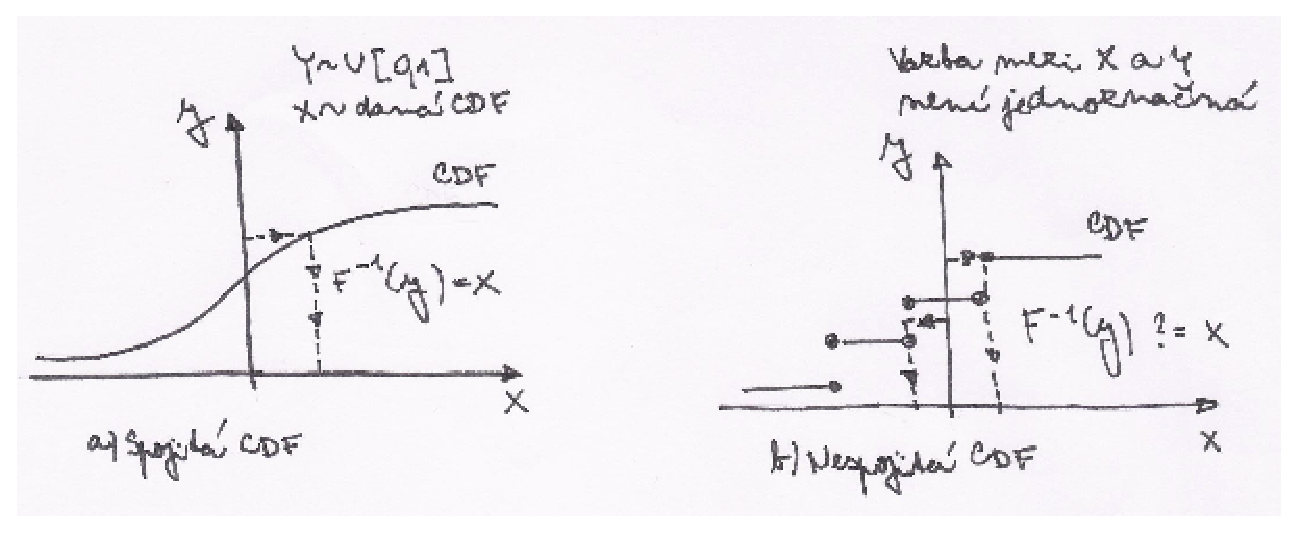
\includegraphics[scale = 0.5]{pictures/inv_cdf.eps}
\caption{Inverze kumulativní distribuční funkce}
\label{inv_cdf}
\end{figure} 

\subsection{Sklarova věta}

Libovolná distribuční funkce definovaná nad $R^d$ v sobě implicitně zahrnuje kopula funkci. Toto tvrzení platí také naopak. Jestliže ``spojíme'' kopula funkci a marginální cdf, získáme vícerozměrné rozdělení. Toto tvrzení vyplývá z následující věty.

\begin{theorem}[Sklarova věta]
Uvažujme $d$-rozměrnou distribuční funkci $F$ s marginálními distribučními funkcemi $F_1, ..., F_d$. Pak existuje kopula funkce taková, že
\begin{equation}
F(x_1, ..., x_d) = C\big(F_1(x_1), ..., F_d(x_d)\big)
\end{equation}
pro všechna $x_i$ v $(-\infty, \infty)$, $i = 1, ..., d$. Jestliže je $F_i$ spojitá pro všechna $i = 1, ..., d$, pak je $C$ jedinečné. V opačném případě je $C$ jedinečné pouze na $Ran(F_1) \times \cdots \times Ran(F_d)$, kde $Ran(F_i)$ označuje obor hodnot distribuční funkce $F_i$\footnote{Např. pro hrací kostku je obor hodnot příslušné distribuční funkce definován jako $\{\frac{1}{6}, \frac{2}{6}, ..., \frac{6}{6}\}$.}.

Výše uvedené tvrzení platí i naopak. Uvažujme kopula funkci $C$ a jednorozměné distribuční funkce $F_1, ..., F_d$. Pak $F$ definovaná dle (1.3) je vícerozměrnou distribuční funkcí s marginálními distribučními funkcemi $F_1, ..., F_d$.
\end{theorem}
S využitím vztahu $F_i \circ F_i^{\leftarrow}(y) \ge y$ získáváme
\begin{equation}
C(u) = F\big(F_1^{\leftarrow}(u_1), ..., F_d^{\leftarrow}(u_d)\big)
\end{equation}
Zatímco (1.3) je zpravidla výchozím bodem pro simulaci, vztah (1.4) slouží spíše pro ``oddělení'' kopula funkce od vícerozměrné distribuční funkce.

\subsection{Hustota pravděpodobnosti kopule}

Dle definice je kopula funkce distribuční funkcí. Vzhledem k obtížné interpretaci kumulativní distribuční funkce se často používá hustota pravděpodobnosti (pdf - probability density function). Je však třeba zmínit, že ne všechny kopula funkce mají odpovídající hustotu pravděpodobnosti. Nicméně má-li kopula funkce diferenci požadovaného řádu, lze hustotu pravděpodobnosti vyjádřit jako
\begin{equation*}
c(u) := \frac{\partial^d C(u_1, ..., u_d)}{\partial u_1, ..., u_d}
\end{equation*}

Jestliže lze kopula funkci vyjádřenou ve tvaru (1.4) derivovat, což má za následek $F_i^{\leftarrow} = F_i^{-1}$, lze odpovídající hustotu pravděpodobnosti vyjádřit jako
\begin{equation*}
c(u) = \frac{f\big(F_1^{-1}(u_1), ..., F_d^{-1}(u_d)\big)}{f_1\big(F_1^{-1}(u_1)\big) \cdots f_d\big(F_d^{-1}(u_d)\big)}
\end{equation*}
kde $f$ označuje sdruženou hustotu pravděpodobnosti a $f_i, i = 1, ..., d$ marginální hustotu pravděpodonosti jednotlivých náhodných veličin.
\begin{proof}
S využitím pravidla pro derivaci složené funkce (chain rule)
\begin{equation*}
\frac{d f(g(x))}{dx} = \frac{df}{dg}\frac{dg}{dx} = f'(g(x))g'(x)
\end{equation*}
a skutečností $F(F^{-1}(u)) = u$ a $\frac{du}{du} = 1$, lze snadno dokázat
\begin{equation*}
\frac{dF(F^{-1}(u))}{du} = f(F^{-1}(u))\frac{dF^{-1}(u)}{du} = 1
\end{equation*}
z čehož vyplývá
\begin{equation*}
\frac{dF^{-1}(u)}{du} = \frac{1}{f(F^{-1}(u))}
\end{equation*}
Derivací dvourozměné kopule funkce ve tvaru (1.4) tak získáme
\begin{multline*}
\frac{dF\big(F_1^{-1}(u_1),F_2^{-2}(u_2)\big)}{du_1du_2} = f\big(F_1^{-1}(u_1), F_2^{-1}(u_2)\big)\frac{F_1^{-1}(u_1)}{du_1}\frac{F_2^{-1}(u_2)}{du_2}\\
= \frac{f\big(F_1^{-1}(u_1), F_2^{-1}(u_2)\big)}{f_1\big(F_1^{-1}(u_1)\big)f_2\big(F_2^{-1}(u_2)\big)}
\end{multline*}
\end{proof}

\subsection{Podmíněné rozdělení}

Uvažujme dvě uniformní náhodné veličiny $U_1$ a $U_2$. Předpokládejme, že známe kopula funkci $C$ a hodnotu náhodné veličiny $U_1$. Cílem je odvodit podmíněné rozdělení, které lze použít pro odhad náhodné veličiny $U_2$. Za předpokladu dostatečné regularity lze odvodit podmíněnou distribuční funkci.
\begin{multline*}
P(U_2 \le u_2 | U_1 = u_1) = \lim_{\delta \rightarrow 0}\frac{P(U_2 \le u_2, U \in (u_1 - \delta, u_1 + \delta])}{P(U_1 \in (u_1 - \delta, u_1 + \delta])}\\
= \lim_{\delta \rightarrow 0}\frac{C(u_1 + \delta, u_2) - C(u_1 - \delta, u_2)}{2 \delta} = \frac{\partial C(u_1, u_2)}{\partial u_1}
\end{multline*}
Podmíněné distribuční funkce lze tedy odvodit derivací kopula funkce $C$ dle $u_1$. Odpovídající podmíněnou hustotu pravděpodobnosti lze získat následnou derivací dle $u_2$.

\subsection{Hraniční hodnoty kopule}

\begin{proposition}
Uvažujme náhodné veličiny $X_1, ..., X_d$, jejichž závislost je definovaná kopula funkcí $C$. Nechť $T_i: R \rightarrow R, i = 1, ..., d$ je striktně rostoucí funkcí. Pak je závislost náhodných veličin $T_1(X_1), ..., T_d(X_d)$ definována toutéž kopula funkcí $C$. 
\end{proposition}
Jinými slovy, striktně rostoucí transformace nemění strukturu závislosti, což se na první podhled může zdát kontraintuitivní. Monotonní transformace totiž sice mění závislost mezi náhodnými veličinami, nicméně po očištění o vliv marginálních distribučních funkcí získáme shodnou strukturu závislosti definovanou kopula funkcí $C$.

Hoeffding a Fréchet nezávisle na sobě odvodili, že kopula funkce vždy leží v rámci určitých hraničních hodnot. Důvody lze nalézt při zkoumání extrémních případů závislosti.
Uvažujme dvě náhodné veličiny $U_1$ a $U_2$. Jestliže $U_1 = U_2$, pak hovoříme o tzv. komonotonických (comonotic) náhodných veličinách a jejich kopula funkce je dána vztahem
\begin{equation}
C(u_1, u_2) = P(U_1 \le u_1, U_1 \le u_2) = min(u_1, u_2)
\end{equation}
Tento typ kopule získéme vždy, když $X_2 = T(X_1)$, kde $T$ je monotonní transformace.
V případě, kdy jsou $U_1$ a $U_2$ nezávislé, je kopula funkce rovna
\begin{equation}
C(u_1, u_2) = u_1 u_2
\end{equation}
Dalším extrémní situací je $U_2 = 1 - U_1$, kdy hovoříme o tzv. kontramonotonických (countermonotonic) náhodných veličinách. Kopula funkce pro $1 - u_2 < u_1$ je
\begin{multline}
C(u_1, u_2) = P(U_1 \le u_1, U_2 \le u_2) = P(U_1 \le u_1, 1 - U_1 \le u_2)\\
= P(U_1 \le u_1, U_1 \ge 1 - u_2) = P(1 - u_2 \le U_1 \le u_1)\\
= u_1 - (1 - u_2) = u_1 + u_2 - 1
\end{multline}
Výše uvedené lze rozšířit na vícerozměrné rozdělení. Ačkoliv komonotonická kopule existuje pro libovolnou dimenzi $d$, kontramonotonická kopule existuje pouze pro $d = 2$\footnote{Uvažujme náhodné veličiny $X_1$, $X_2$ a $X_3$. Jako kontramonotonické zvolme páry $(X_1, X_2)$ a $(X_1, X_3)$. Tato volba představuje omezení pro závislost mezi $X_2$ a $X_3$. Jestliže se $X_1$ sníží, jak $X_2$ tak $X_3$ se musí zvýšit a tudíž nemohou být kontramonotonické.}, nicméně hraniční hodnoty jsou platné i pro vyšší dimenze.

\begin{theorem}[Fréchet-Hoeffdingovy hraniční hodnoty]
Uvažujme kopula funkci $C(u) = C(u_1, ..., u_d)$. Pak platí
\begin{equation*}
\max\left(\sum_{i = 1}^d u_i + 1 - d, 0 \right) \le C(u) \le \min\left(u_1, ..., u_d\right)
\end{equation*}
\end{theorem}

\begin{figure}[htp]
\centering
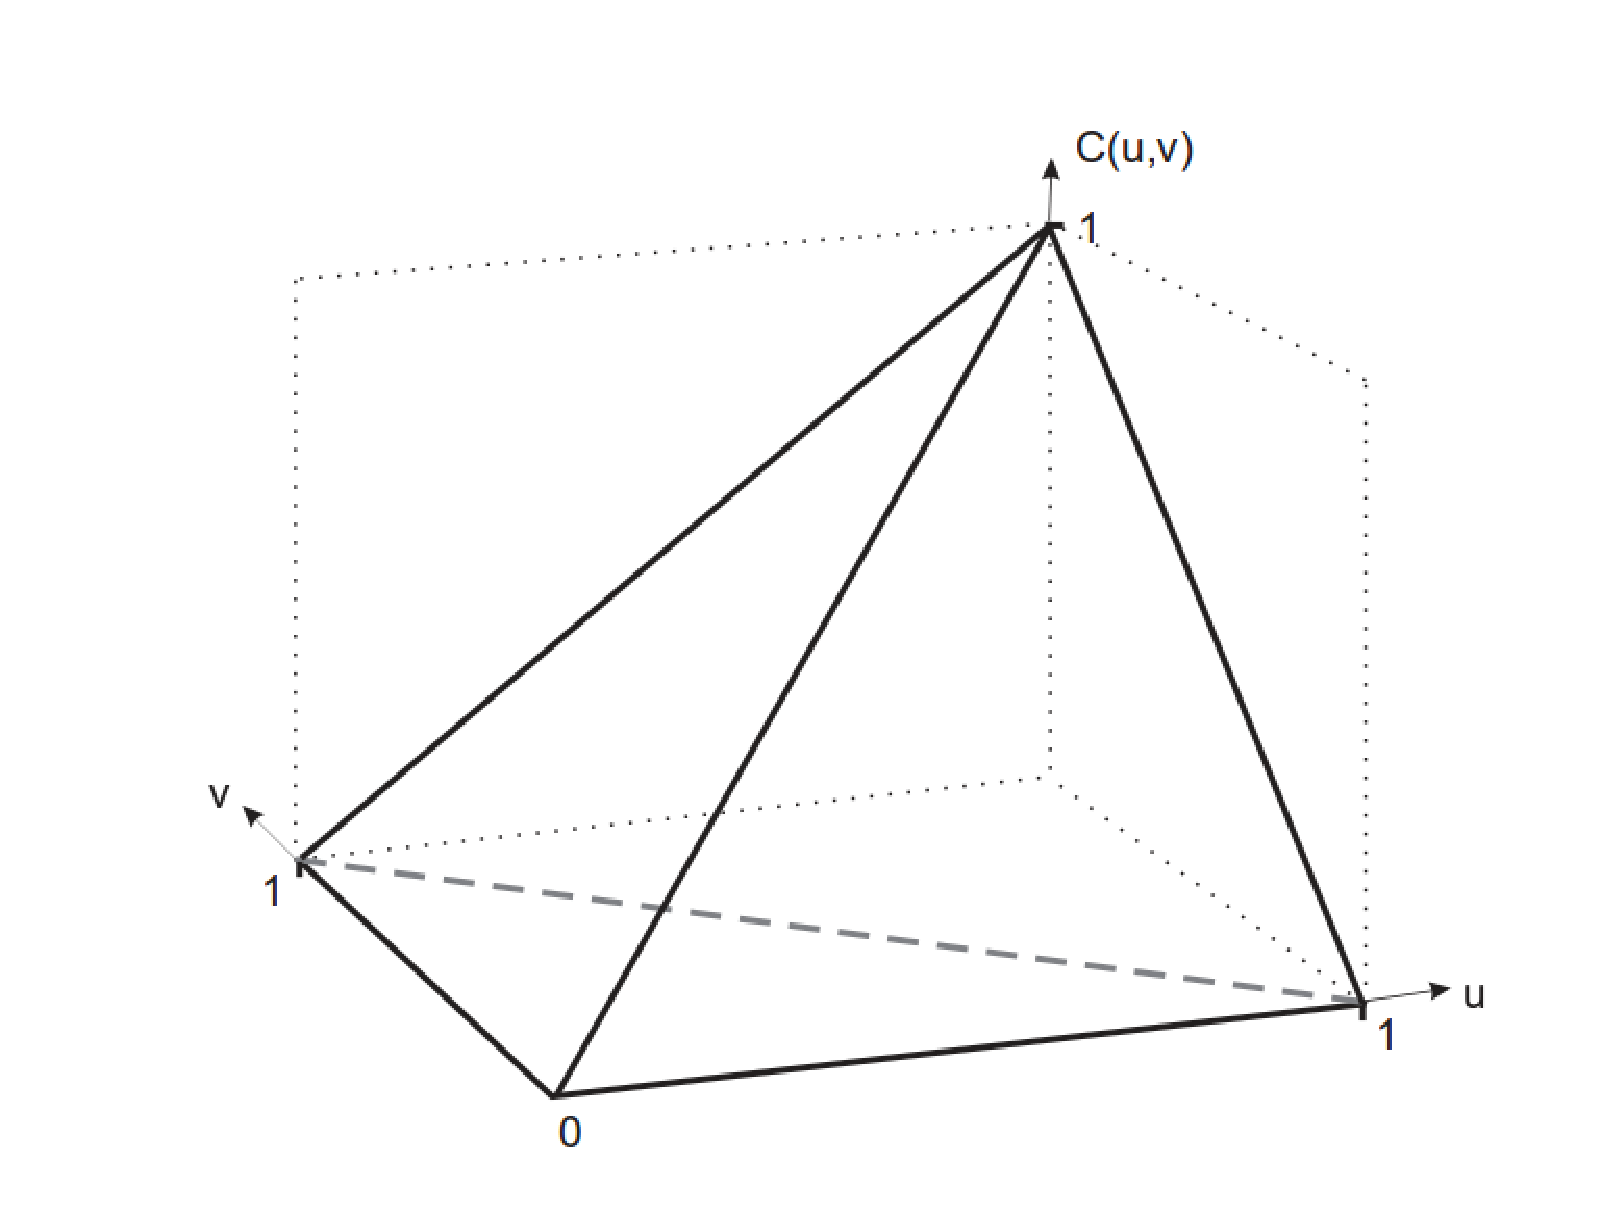
\includegraphics[scale = 0.35]{pictures/copula_boundary.eps}
\caption{Fréchet-Hoeffdingovy hraniční hodnoty - Každá kopula funkce leží uvnitř zobrazené pyramidy. Povrch daný spodní a zadní stěnou pyramidy (dolní hranice) představuje kontramonotonistickou kopula funkcí $C(u, v) = \max\{u + v -1, 0\}$. Povrch daný přední stěnou pyramidy (horní hranice) pak představuje monotonostickou kopula funkci $C(u, v) = \min(u, v)$.}
\label{copula_boundary}
\end{figure} 

\chapter{Míra závislosti}

\section{Korelace}

Korelace $\rho(X_1, X_2)$ mezi náhodnými veličinami $X_1$ a $X_2$ je definována jako
\begin{equation*}
\rho(X_1, X_2) = \frac{cov(X_1, X_2)}{\sqrt{D(X_1)D(X_2)}}
\end{equation*}
kde
\begin{equation*}
cov(X_1, X_2) = E[(X_1 - E[X1])(X_2 - E[X_2])]
\end{equation*}
Korelace vyjadřuje míru lineární závislosti a nabývá hodnot z intervalu $[-1, 1]$. Jestliže jsou $X_1$ a $X_2$ nezávislé, pak $\rho(X_1, X_2) = 0$. Opačné trvzení však neplatí - pokud je korelace rovna nula, neznamená to, že jsou $X_1$ a $X_2$ nezávislé. Pokud $|\rho(X_1, X_2)| = 1$ jsou $X_1$ a $X_2$ dokonale lineárně korelované, což znamená, že $X_2 = \alpha + \beta X_1$ téměř jistě pro některé $\alpha \in R$ a $\beta \neq 0$\footnote{V případě $\beta > 0$ hovoříme o pozitivní lineární korelaci. V případě $\beta < 0$ hovoříme o negativní lineární korelaci.}. Pro $\beta_1, \beta_2 > 0$ navíc platí
\begin{equation*}
\rho(\alpha_1 + \beta_1 X_1, \alpha_2 + \beta_2 X_2) = \rho(X_1, X_2)
\end{equation*}
což znamená, že korelace je invariantní pro striktně rostoucí lineární transformaci. Nicméně je třeba zdůraznit, že korelace není invariantní pro nelineární striktně rostoucí trasformaci $T: R \rightarrow R$. Pro dvě náhodné veličiny tedy obecně platí $\rho(T(X_1), T(X_2)) \neq rho(X_1, X_2)$.

\begin{fallacy}
Sdružená distribuční funkce je jednoznačně definována pomocí marginálních distribučních funkcí a párových korelací.
\end{fallacy}

Toto tvrzení je platné pouze v případě vícerozměrných eliptických rozdělení. Kdyby toto tvrzení bylo platné obecně, nebylo by zapotřebí konceptu kopula funkce.

\begin{example}
Uvažujme dvě náhodné veličiny představující zisk / ztrátu dvou portfolií. Předpokládejme, že obě rizika sledují standardní normální rozdělení a že jejich korelace je rovna nule. Zkonstruujme dva náhodné vektory v souladu s těmito předpoklady.

Uvažujme dvě modelové situaci. Model 1 je standardní dvourozměrné normální rozdělení $X \sim N_2(0, I_2)$. V modelu 2 nezávislá náhodná veličina $V$ s pravděpodobnostní funkcí $P(V = 1) = P(V = -1) = \frac{1}{2}$ použita při konstrukci nových náhodných veličin $(Y_1, Y_2) = (X_1, VX_1)$, kde $X_1$ je převzato z modelu 1. Marginální distribuční funkce náhodných veličin $Y_1$ a $Y_2$ sledují taktéž standardní normální rozdělení s nulovou korelací. Kopula funkce modelu 2 je
\begin{equation*}
C(u_1, u_2) = \frac{1}{2} \max(u_1 + u_2 - 1, 0) + \frac{1}{2}\min(u_1, u_2)
\end{equation*}
což je mix dvourozměrných kopula funkcí s Fréchetovou hraniční hodnotou. Náhodné velčiny $Y_1$ a $Y_2$ tedy nejsou nezávislé.
\end{example}

\begin{fallacy}
Pro libovolné jednorozměrné distribuční funkce $F_1$ a $F_2$ a libovolnou korelaci $\rho$ z intervalu $[-1, 1]$ je vždy možné zkonstruovat sdruženou distribuční funkci $F$ s marginálními distribučními funkcemi $F_1$ a $F_2$ a korelací $\rho$.
\end{fallacy}

Toto tvrzení je opět platné pouze pro eliptické pravděpodobnostní rozdělení. Tzv. dosažitelné korelace mohou tvořit podmnožinu intervalu $[-1, 1]$.

\begin{proposition}
Jestliže $(X_1, X_2)$ sleduje sdruženou distribuční funkci $F$ a marginální distribuční funkce $F_1$ a $F_2$, pak je kovariance $X_1$ a $X_1$, pokud je konečná, dána vztahem
\begin{equation}
cov(X_1, X_2) = \int_{-\infty}^{\infty} \int_{-\infty}^{\infty}(F(x_1, x_2) - F_1(x_1)F_2(x_2))dx_1 dx_2
\end{equation}
\end{proposition}

\begin{proof}
Nechť $(X_1, X_2)$ sleduje sdruženou distribuční funkci $F$ a nechť $(\tilde{X}_1, \tilde{X}_2)$ je její nezávislou kopií\footnote{Jedná se tedy o druhý pár, který sleduje sdruženou distribuční funkci $F$ a který je nezávislý na $(X_1, X_2)$.}. Platí
\begin{multline*}
E[(X_1 - \tilde{X}_1)(X_2 - \tilde{X}_2)] = E[X_1X_2 - X_1\tilde{X}_2 - \tilde{X}_1X_2 + \tilde{X}_1 \tilde{X}_2]\\
= E[X_1X_2] - E[X_1 \tilde{X}_2] + E[\tilde{X}_1 \tilde{X}_2] - E[\tilde{X}_1X_2]\\
= E[X_1X_2] - E[X_1]E[X_2] + E[X_1X_2] - E[X_1]E[X_2]\\
= 2 cov(X_1, X_2)
\end{multline*}
Nyní použijme identitu, která říká, že pro libovolné $a \in R$ a $b \in R$ platí $(a - b) = \int_{-\infty}^{\infty}(I_{\{b \le x\}} - I_{\{a \le x\}})dx$, a aplikujeme ji na $(X_1 \tilde{X}_2)$ a $(X_2 - \tilde{X}_2)$. Získáme
\begin{multline*}
2cov(X_1, X_2)\\
= E\left[\int_{-\infty}^{\infty}\int_{-\infty}^{\infty}\left(I_{\{\tilde{X}_1 \le x_1\}} - I_{\{X_1 \le x_1\}}\right)\left(I_{\{\tilde{X}_2 \le x_2\}} - I_{\{X_2 \le x_2\}}\right)dx_1 dx_2\right]\\
= 2 \int_{-\infty}^{\infty}\int_{-\infty}^{\infty} \left(P(X_1 \le x_1, X_2 \le x_2) - P(X_1 \le x_1)P(X_2 \le x_2)\right)dx_1 dx_2
\end{multline*}
\end{proof}
\begin{theorem}[Dosažitelné korelace]
Nechť je $(X_1, X_2)$ náhodný vektor s marginálními distribučními funkce $F_1$ a $F_2$, které mají nenulový konečný rozptyl\footnote{Tj. předpokládáme, že $0 < D(X_1) < \infty$ a $0 < D(X_2) < \infty$.}, a blíže nespecifikovanou sdruženou distribuční funkcí. Pak platí následující tvrzení
\begin{enumerate}
\item Dosažitelné korelace formují uzavřený interval $[\rho_{min}, \rho_{max}]$, kde $\rho_{min} < 0 < \rho_{max}$.
\item Minimální korelace $\rho_{min}$ je dosažena pouze v případě kontramonotonocity $X_1$ a $X_2$. Maximální korelace $\rho_{max}$ je dosaženo pouze jsou-li $X_1$ a $X_2$ komonotonické.
\item Krajních hodnot $\rho_{min} = -1$ a $\rho_{max} = 1$ lze dosáhnout pouze tehdy a jen tehdy jsou-li $X_1$ a $-X_2$ téhož typu\footnote{Dvě náhodné veličiny $V$ a $W$ jsou stejného typu, jestliže existují konstanty $a > 0$ a $b \in R$ takové, že $V = aW + b$. Jinými slovy pravděpodobnostní rozdělení stejného typu lze získat jedno z druhého pomocí lokace a transformací měřítka.}.
\end{enumerate}
\end{theorem}

\begin{proof}
Začněme trvzením (2) a identitou (2.1). Připomeňme si, že dvourozměrná kopula funkce je omezena hraničními podmínkami
\begin{equation*}
max(F_1(x_1) + F_2(x_2) - 1, 0) \le F(x_1, x_2) \le min(F_1(x_1). F_2(x_2))
\end{equation*}
Pokud jsou $F_1$ a $F_2$ dané, je integrand v (2.1) maximalizován pro hraniční hodnotu $min(F_1(x_1), F_2(x_2))$, tj. v případě komonotonické kopula funkce. Analogicky je integrand minimalizován v případě kontramonotonické kopula funkce $max(F_1(x_1) + F_2(x_2) - 1, 0)$. Pro maximálně dosažitelnou korelaci platí $\rho_{max} \ge 0$. Nicméně $\rho_{max} = 0$ můžeme vyloučit, protože to by implikovalo $min(F_1(x_1), F_2(x_2)) = F_1(x_1)F_2(x_2)$ pro všechna $x_1$ a $x_2$. To by však vyžadovalo, aby $F_1$ a $F_2$ byly degenerované distribuční funkce s pravděpodobností koncentrovanou v jednou bodě. To je však vyloučeno předpokladem nenulového rozptylu. Podobnými argumenty lze prokázat $\rho < 0$. Jestliže pomocí $W(F_1, F_2)$ resp. $M(F_1, F_2)$ označíme Fréchetovu dolní resp. horní hraniční hodnotu, pak kopula funkce $\lambda W(F_1, F_2) + (1 - \lambda)M(F_1, F_2)$ pro $0 \le \lambda \le 1$ implikuje korelaci $\lambda \rho_{min} + (1 - \lambda)\rho_{max}$. Pro libovolné $\rho \in [\rho_{min}, \rho_{max}]$ tak získáváme $\lambda = \frac{\rho_{max} - rho}{\rho_{max} - \rho_{min}}$.

Tvrzení (3) je zřejmé, protože $\rho_{min} = -1$ popř. $\rho_{max} = 1$ pouze tehdy a jen tehdy je-li mezi $X_1$ a $X_2$ téměř jistě nelineární vztah.
\end{proof}

\begin{example}[Dosažitelná korelace pro lognormální náhodné veličiny]
Předpokládejme, že $\ln(X_1) \sim N(0, 1)$ a $\ln(X_2) \sim N(0, \sigma^2)$. Pro $\sigma \ne 1$ nejsou $X_1$ a $X_2$ shodného typu (ačkoliv $\ln(X_1)$ a $\ln(X_2)$ jsou), a proto dle bodu (3) výše uvedené věty platí $\rho_{max} < 1$. Náhodné veličiny $X_1$ a $-X_2$ taktéž nejsou stejného typu, a proto opět platí $\rho_{min} > -1$.

Definujme $Z \sim N(0, 1)$ a všimněme si, že pokud jsou $X_1$ a $X_2$ komonotické, pak $(X_1, X_2) =^d (e^Z, e^{\sigma Z})$. Je zřejmé, že $\rho_{max} = \rho(e^Z, e^{\sigma Z})$. Analogicky lze dovodit $\rho_{min} = \rho(e^Z, e^{-\sigma Z})$. Analyckým řešením těchto dvou vztahů lze odvodit
\begin{equation*}
\rho_{min} = \frac{e^{-\sigma} - 1}{\sqrt{(e - 1)(e^{\sigma^2} - 1)}}, ~~~ \rho_{max} = \frac{e^{\sigma} - 1}{\sqrt{(e - 1)(e^{\sigma^2} - 1)}}
\end{equation*}
\end{example}

Výše uvedený text lze z praktického hlediska shrnout do konstatování, že koncept korelace je bezobsažný, pokud není aplikován v kontextu řádně specifikovaného spojitého modelu.

\section{Pořadová korelace}

Pořadová korelace je měřítko závislosti, které je závislé pouze na dvourozměrné kopula funkci a nikoliv na marginálních distribučních funkcí. Připomeňme, že lineární korelace je závislá jak na kopula funkci, tak na marginálních distribučních funkcích. V praxi jsou jako měřítko pořadové korelace používány Kendallova a Spearmanova korelace.

\subsection{Kendallova korelace}

Kendalovu pořadovou korelaci je možné chápat jako měřítko shody pro dvourozměrné náhodné vektory. Dva body v $R^2$ označené jako $(x_1, x_2)$ a $(\tilde{x}_1, \tilde{x}_2)$ jsou ve shodě, jestliže $(x_1 - \tilde{x}_1)(x_2 - \tilde{x}_2) > 0$. Uvažujme dva náhodné vektory $(X_1, X_2)$ a $(\tilde{X}_1, \tilde{X}_2)$ z téhož pravděpodobnostního rozdělení. Jestliže má $X_2$ tendenci růst s $X_1$, pak očekáváme, že četnost shody $(x_1 - \tilde{x}_1)(x_2 - \tilde{x}_2) > 0$ bude relativně vyšší než neshody $(x_1 - \tilde{x}_1)(x_2 - \tilde{x}_2) < 0$. Analogické tvrzení platí také naopak. Tato myšlenka stojí za Kendallovou pořadovou korelací, která je definována jako rozdíl odpovídajících pravděpodobností, tj.
\begin{equation}
\rho_{\tau}(X_1, X_2) = P\left((X_1 - \tilde{X}_1)(X_2 - \tilde{X}_2) > 0 \right) - P\left((X_1 - \tilde{X}_1)(X_2 - \tilde{X}_2) < 0 \right)
\end{equation}
nebo-li
\begin{equation*}
\rho_{\tau}(X_1, X_2) = E\left[sign\left((X_1 - \tilde{X}_1)(X_2 - \tilde{X}_2)\right)\right]
\end{equation*}
kde $sign(x) = -1$ pro $x < 0$, $sign(x) = 0$ pro $x = 0$ a $sign(x) = 1$ pro $x > 0$.

Související funkce \textit{CalcKendallTau.m} je k dispozici v adresáři \textit{libs}.

\subsection{Spearmanova korelace}

\begin{definition}
Pro dvě náhodné veličiny $X_1$ a $X_2$ s marginálními distribučními funkcemi $F_1$ a $F_2$ je Spearmanova korelace definována jako
\begin{equation*}
\rho_S(X_1, X_2) = \rho(F_1(X_1), F_2(X_2))
\end{equation*}
\end{definition}

\subsection{Vlastnosti pořadové korelace}

Jak Kendallova tak Spearmanova korelace jsou symetrická měřítka závislosti, které nabývají hodnot z intervalu $[-1, 1]$. Pro nezávislé náhodné veličiny nabývají nulové hodnoty, nicméně, podobně jako u lineární korelace, nulová pořadová korelace neimplikuje nezávislé náhodné veličiny. Lze také dokázat, že pořadová korelace nabývá hodnoty 1 pro komonotonické náhodné veličiny a hodnoty -1 pro kontramonotonotické náhodné veličiny.

Následující odstavec tvrdí, že pro spojité marginální distribuční funkce, obě pořadové korelace závisí pouze na kopule funkci, a proto sdílejí její vlastnost invariance pro monotónně rostoucí transformaci.

\begin{proposition}
Předpokládejme, že $X_1$ a $X_2$ mají spojité marginální distribuce a jedinečnou kopula funkci $C$. Pořadové korelace jsou pak dány
\begin{multline}
\rho_{\tau}(X_1, X_2) = 4 \int_0^1 \int_0^1 C(u_1, u_2)dC(u_1, u_2) - 1\\
\rho_S(X_1, X_2) = 12 \int_0^1 \int_0^1 (C(u_1, u_2) - u_1 u_2)du_1 du_2
\end{multline}
\end{proposition}

\begin{proof}
Z (2.2) lze snadno odvodit, že Kendallovu korelaci lze také vyjádřit jako
\begin{equation*}
\rho_{\tau}(X_1, X_2) = 2 P((X_1 - \tilde{X}_1)(X_2 - \tilde{X}_2) > 0) - 1
\end{equation*}
a ze vzájemné zaměnitelnosti párů $(X_1, X_2)$ a $(\tilde{X}_1, \tilde{X}_2)$ vyplývá
\begin{multline}
\rho_{\tau}(X_1, X_2) = 4 P(X_1 < \tilde{X}_1, X_2 < \tilde{X}_2) - 1\\
= 4 E(P(X_1 < \tilde{X_1}, X_2 < \tilde{X}_2 | \tilde{X_1}, \tilde{X_2})) - 1\\
= 4 \int_{-\infty}^{\infty} \int_{-\infty}^{\infty}P(X_1 < x_1, X_2 < x_2)dF(x_1, x_2) - 1
\end{multline}
Protože $X_1$ a $X_2$ mají spojité marginální distribuční funkce, platí
\begin{equation*}
\rho_{\tau}(X_1, X_2) = \int_{-\infty}^{\infty} \int_{-\infty}^{\infty} C(F_1(x_1), F_2(x_2)) dC(F_1(x_1), F_2(x_2)) - 1
\end{equation*}
z čehož po dosazení $u_1 := F_1(x_1)$ a $u_2 := F_2(x_2)$ vyplývá (2.3).

Pro odvození (2.4) je klíčové si uvědomit, že $F_i(X_i)$ sleduje uniformní rozdělení nad intervalem $[0, 1]$ s rozptylem $\frac{1}{12}$. To má za následek $\rho_S(X_1, X_2) = 12 cov(F_1(X_1), F_2(X_2))$. Vztah (2.4) pak získáme přímou aplikací (2.1).
\end{proof}

Omyl (1), který jsme zmiňovali v souvislosti s lineární korelací, je relevantní také pro pořadovou korelaci - marginální distribuční funkce a pořadová korelace plně nedefinují vícerozměrné pravděpodobnostní rozdělení. Možnost omylu (2) však v případě pořadové korelace odpadá - pro libovolné marginální distribuční funkce je možné definovat dvourozměrné pravděpodobnostní rozdělení, které má požadovanou pořadovou korelaci z intervalu $[-1, 1]$. Jedním ze způsobů jak toho docílit je výše představená kombinace kontramonotonotické a komonotonické kopula funkce
\begin{equation*}
F(x_1, x_2) = \lambda W(F_1(x_1), F_2(x_2)) + (1 - \lambda)M(F_1(x_1), F_2(x_2))
\end{equation*}
Náhodný pár $(X_1, X_2)$ s touto kopula funkcí má pořadovou korelaci
\begin{equation*}
\rho_{\tau}(X_1, X_2) = \rho_S(X_1, X_2) = 1 - 2 \lambda
\end{equation*}

\subsection{Koeficienty závislosti v chvostech}

Koeficienty závislosti v chvostech měří, jak jejich název napovídá, míru závislosti v chvostech dvourozměrného pravděpodobnostního rozdělení. Koeficienty, které si popíšeme v následujím textu, jsou definovány jako limitní podmíněné pravděpodobnosti v chvostu definovaného extrémním kvantilem.

\begin{definition}
Nechť $X_1$ a $X_2$ jsou náhodné veličiny s marginálními distribučními funkcemi $F_1$ a $F_2$. Koeficient závislosti v horním chvostu je definován
\begin{equation*}
\lambda_u := \lambda_u (X_1, X_2) = \lim_{q \rightarrow 1^-}P\left(X_2 > F_2^{\leftarrow}(q) | X_1 > F_1^{\leftarrow}(q)\right)
\end{equation*}
za předpokladu existence limitu $\lambda_u \in [0, 1]$. Je-li $\lambda_u \in (0, 1]$, říkáme o $X_1$ a $X_2$, že vykazují závislost z horním chvostu; $\lambda_u = 0$znamená, že $X_1$ a $X_2$ jsou v horním chvostu asymptoticky nezávislé. Analogicky koeficient závislosti v dolním chvostu je definován jako
\begin{equation*}
\lambda_l := \lambda_l(X_1, X_2) = \lim_{q \rightarrow 0^+} P \left(X_2 \le F_2^{\leftarrow}(q) | X_1 \le F_1^{\leftarrow}(q)\right)
\end{equation*}
za předpokladu existence $\lambda_l \in [0, 1]$.
\end{definition}

Pokud jsou distribuční funkce $F_1$ a $F_2$ spojité, lze $\lambda_u$ a $\lambda_l$ vyjádřit pomocí kopula funkce jako
\begin{multline*}
\lambda_l = \lambda_{q \rightarrow 0^+} \frac{P\left(X_2 \le F_2^{\leftarrow}(q), X_1 \le F_1^{\leftarrow}(q)\right)}{P\left(X_1 \le F_1^{\leftarrow}(q)\right)}\\
= \lim_{q \rightarrow 0^+} \frac{C(q, q)}{q}
\end{multline*}
resp. jako
\begin{multline*}
\lambda_u = \lambda_{q \rightarrow 1^-} \frac{P\left(X_2 > F_2^{\leftarrow}(q), X_1 > F_1^{\leftarrow}(q)\right)}{P\left(X_1 > F_1^{\leftarrow}(q)\right)}\\
= \lim_{q \rightarrow 0^+} \frac{\hat{C}(1 - q, 1 - q)}{1 - q} = \lim_{q \rightarrow 0^+} \frac{\hat{C}(q, q)}{q}
\end{multline*}
kde $\hat{C}$ je tzv. kopula funkce přežití (survival copula) definovaná jako
\begin{equation*}
\hat{C}(1 - u_1, 1 - u_2) = 1 - u_1 - u_2 + C(u_1, u_2)
\end{equation*}
Pro radiálně symetrické kopula funkce platí $\lambda_l = \lambda_u$, protože v jejich případě $C = \hat{C}$.

\begin{example}[Gumbelova kopulace funkce]
Gumbelova kopulace funkce je defivána jako $C_{\theta}^{Gu} = e^{-((-\ln(u_1))^{\theta} + (-\ln(u_2))^{\theta})^{1/\theta}}, ~~~ 1 \le \theta < \infty$. Koecifient závislosti v horním chvostu je tedy dán vztahem
\begin{equation*}
\lambda_u = \lim_{q \rightarrow 1^-} \frac{\hat{C}_{\theta}^{Gu}(1 - q, 1 - q)}{1 - q} = 2 - \lim_{q \rightarrow 1^-} \frac{C_{\theta}^{Gu}(q, q) - 1}{q - 1}
\end{equation*}
S využitím L'Hospitalova pravidla a skutečnosti $C_{\theta}^{Gu}(u, u) = u^{2^{1 / \theta}}$ lze dovodit
\begin{equation*}
\lambda_u = 2 - \lim_{q \rightarrow 1^-} \frac{dC_{\theta}^{Gu}(q, q)}{dq} = 2 - 2 ^ {1 / \theta}
\end{equation*}
Pro $\theta > 1$ tedy Gumbelova kopula funkce vykazuje závilost v horním chvostu. Síla této závoslosti se limitně blíží 1 s tím, jak $\theta \rightarrow \infty$. To v souladu s intuicí, protože pro $\theta \rightarrow \infty$ se Gumbelova kopula funkce stáva komonotonickou kopula funkcí.
\end{example}

Kód pro výpočet závoslosti v chvostech dvourozměrné kopula funkce je k dispozici v adresáři \textit{Copulas} ve funkci \textit{CopulaTailDependence}.

\chapter{Odhad kopula funkce}

Koncept kopule zahrnuje několik podkladových funkcí - marginální distribuční funkce jednotlivých náhodných veličin a kopula funkci, která popisuje závilost jejich kvantilů. Protože volba marginální funkce má skrze jí implikované kvantily vliv na volbu kopula funkce, měly by se teoreticky obě odhadovat společně. To je však v praxi poměrně obtížné, a proto odhad zpravidla probíhá ve dvou krocích - v prvním kroku se odhadnou marginální distribuční funkce a ve druhém kroku se hledá kopula funkce, která nejlépe odpovídá kvantilům, které byly vypočteny na základě jednotlivých distribučních funkcí.

\begin{figure}[htp]
\centering
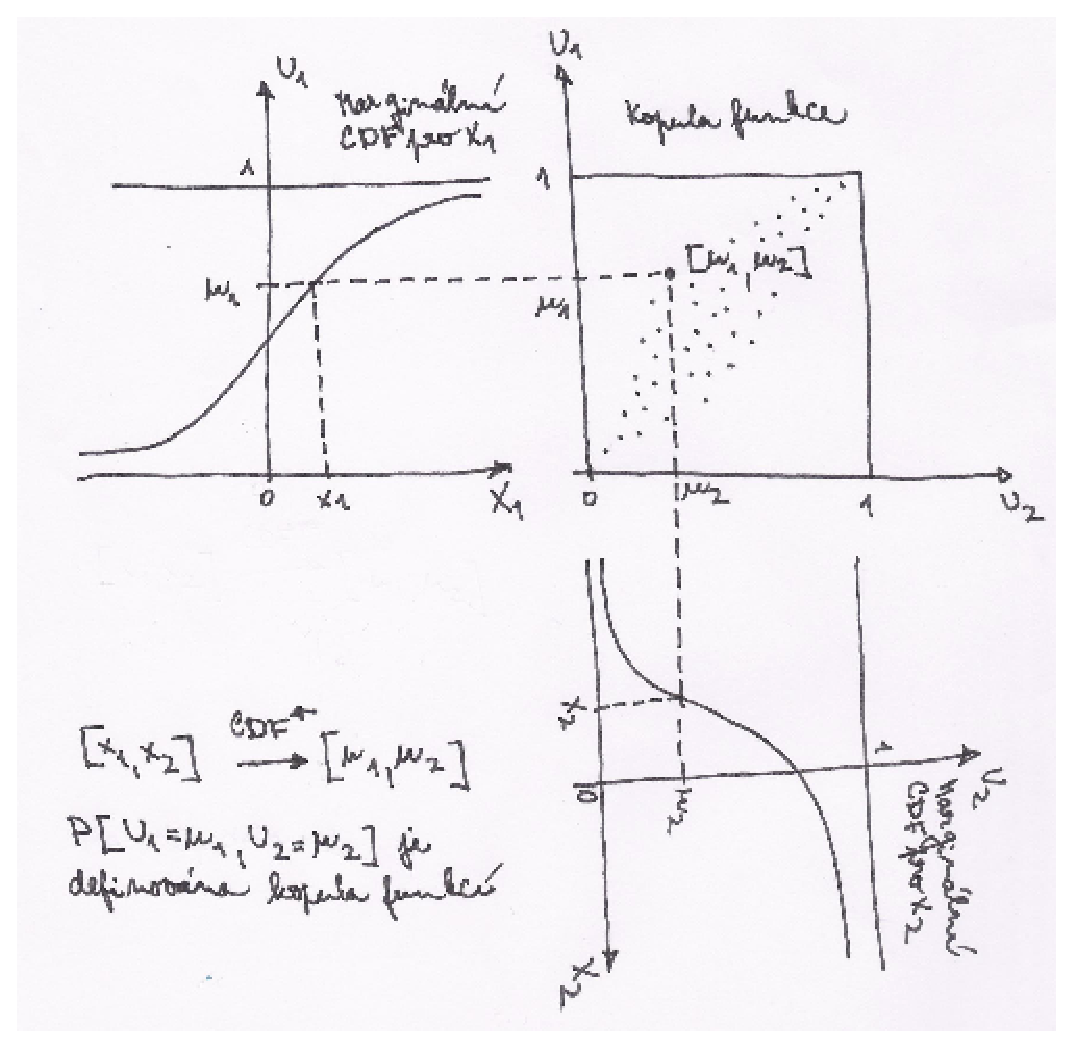
\includegraphics[scale = 0.50]{pictures/copula_concept.eps}
\caption{Koncept kopula funkce}
\end{figure}

\section{Marginální distribuční funkce}

Prvním krokem je odhad marginálních distribučních funkcí, z nichž následně odvodíme kvantily pro jednotlivá pozorování. Marginální distribuční funkce je možné odhadnout několika různými způsoby. Mezi nejběžnější patří následující.
\begin{itemize}
\item Nejjednodušším způsobem je aproximace pomocí empirické distribuční funkce. Nevýhodou tohoto přístupu je, že (a) odhadnutá distribuční funkce je nespojitá, což představuje problém při její inverzi a (b) z důvodu nedostatečného počtu extrémních pozorování nemusí správně odhadovat odlehlé kvantily.
\item Další neparametrický způsob odhadu distribuční funkce spočívá ve využitím jádrového vyhlazení (kernel smoothing) empirických dat. Tento přístup je tedy rozšířením předhozího. Distribuční funkce je, zjednodušeně řečeno, v jednotlivých bodech odhadu aproximována pomocí váženého průměru jednotlivých empirických kvantilů. Výhodou oproti předchozímu přístupu je hladká distribuční funkce, nicméně problém s odlehlými kvantily zůstává.
\item Právě z důvodu problému s odlehlými kvantily je preferován parametrický odhad. V tomto případě se zvolí konkrétní pravděpodobnostní rozdělení, jehož parametry se následně odhadnou na základě empirických dat. Výhodou je hladká distribuční funkce, pro kterou máme zpravidla k dispozici funkční předpis. Na druhou stranu právě z důvodu volby pravděpodobnostního rozdělení zahrnuje tento postup určitou míru subjektivity.
\end{itemize}

Než se zaměříme na jednotlivé způsoby odhadu distribuční funkce, je třeba zdůraznit, že volba marginální distribuční funkce má dopad na výpočet hodnoty kvantilů a tím pádem také na následný odhad kopula funkce. Nevhodný způsob konstrukce marginální distribuční funkce tak může mít fatální důsledky.

\subsection{Empirická distribuční funkce}

Předpokládejme, že máme k dispozici určitý počet pozorovaných hodnot z realizace náhodné veličiny jako je např. logaritmická změna ceny konkrétní akcie obchodované na burze v průběhu určitého období.

Prvním krokem při konstrukci empirické distribuční funkce je rozdělení reálné osy (tj. v našem případě možného cenového rozpětí) na několik disjuktních intervalů. Jejich počet závisí na počtu pozorování, která máme k dispozici - čím více pozorování, tím více může být těchto intervalů. Každé pozorování přiřadíme  s ohledem na jeho hodnotu právě jednomu z těchto intervalů.

Po té, co máme všechna pozorování přiřazena, spočítáme jejich relativní četnost pro jednotlivé intervalech. Délka intervalů nemusí být shodná - v ideálním případě by měla být nastavena tak, aby každý z nich obsahoval přibližně stejný počet pozorování. Tím omezíme velikost ``schodů'' empirické distribuční funkce při přechodu z jednoho intervalu do druhého.

Posledním krokem je postupné načítání relativních četností přes jednotlivé intervaly, čímž získáme empirickou distribuční funkci. Tato funkce je nespojitá, tj. vykazuje ``schody'' při přechodu z jednoho intervalu do druhého. Ačkoliv lze velikost těchto ``schodů'' omezit navýšením počtu pozorování (a s tím souvisejícím větším počtem možných intervalů) popř. vhodnou volbou intervalů (viz. výše), zcela zbavit se jich nelze. Nespojitost empirické distribuční funkce znamená, že neexistuje její inverzní funkce, což je třeba zohlednit při případné simulaci.

Je zřejmé, že kvalita empirické distribuční funkce je silně závislá na počtu pozorování. To platí zejména pro odlehlé kvantily. Jestliže máme např. k dispozici 100 pozorování, nemůžeme na základě empirické distribuční funkce vznášet závěry ohledně kvantilu 0.1\% a 99.9\%. A právě tyto kvantily jsou hlavním předmětem zájmu při řízení finančních rizik, což snižuje použitelnost tohoto přístupu v praxi.

\subsection{Jádrové vyhlazení}

\subsubsection{Popis metody}

Jádrové vyhlazení je statistická technika pro odhad reálné funkce $f(X), X \in R^d$ na základě empirických dat v případech, kdy není znám funkční předpis $f(x)$. Odhadovaná funkce je hladká, přičemž stupeň ``vyhlazení'' je dán jediným parametrem.

Nechť $K_{h_{\lambda}}(X_0, X)$ je jádro definované jako
\begin{equation*}
K_{h_{\lambda}}(X_0, X) = D\left(\frac{\parallel X - X_0\parallel}{h_{\lambda}(X_0)} \right)
\end{equation*}
kde $X, X_0 \in R^d$, $h_{\lambda}(X_0)$ je parametr vyhlazení a $D(t)$ je kladná reálná funkce, jejíž hodnota klesá s rostoucím $\parallel X - X_0\parallel$, tj. vzdáleností mezi body $X$ a $X_0$.
Nechť $\hat{Y}(X): R^d \rightarrow R$ je spojitou funkcí proměnné $X$. Pak pro libovolné $X_0 \in R^d$ je Nadaraya-Watsonův vážený průměr založený na jádře definován jako
\begin{equation*}
\hat{Y}(X_0) = \frac{\sum_{i = 1}^N K_{h_{\lambda}}(X_0, X_i)Y(X_i)}{\sum_{i = 1}^N K_{h_{\lambda}}(X_0, X_i)}
\end{equation*}
kde $N$ je počet pozorování a $Y(X_i)$ je hodnota pozorování v bodě $X_i$.

Existuje řada jader, nicméně nejčastěji používaným je Gausovo jádro. To je definováno jako
\begin{equation*}
K_{h_{\lambda}}(X_0, X) = \frac{1}{\sqrt{2 \pi h^2}} e^{-\frac{1}{2}\left(\frac{\parallel X - X_0\parallel}{h}\right)^2}
\end{equation*}
kde parametr vyhlazení je zpravidla zvolen jako $h = 1.06 \sigma_Y N ^{-\frac{1}{5}}$ s $\sigma_Y$ představující směrodatnou odhylku hodnot pozorování $Y(X_i)$. 

\subsubsection{Aplikace}

Po té, co je na základě pozorování zkonstruována empirická distribuční funkce, lze na tuto funkci aplikovat jádrové vyhlazení. Výhodou jádrového vyhlazení je, že lze empirickou distribuční funkci tabularizovat na libovolně husté stupnici, čímž lze zásadním způsobem eliminovat problém ``schodů''. Výsledná tabulka se následně používá pro inverzi distribuční funkce. Funkce \textit{KernelSmoothing.m} jádrové vyhlazení je k dispozici v adresáři \textit{libs}. 

\begin{figure}[htp]
\centering
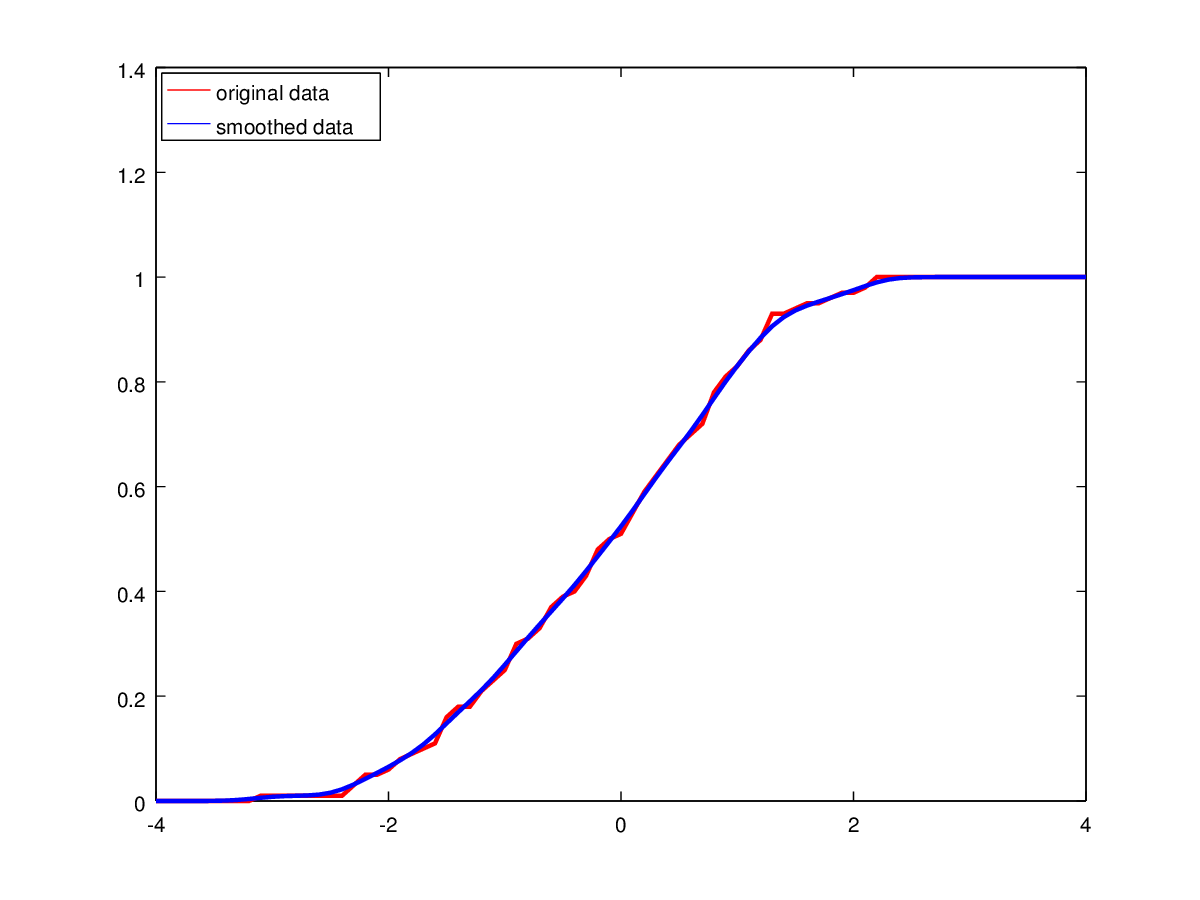
\includegraphics[scale = 0.50]{pictures/kernel_smoothing.eps}
\caption{Vyhlazená empirická distribuční funkce}
\end{figure}

\subsection{Volba pravděpodobnostního rozdělení}

Ve finační teorii se velmi často používá vybraná rodina pravděpodobnostních rozdělení pro popis chování určitých finanční veličin. Nejpopulárnější je normální rozdělení, které se používá pro popis logaritmických změn cen akcií a měnových kurzů nebo absolutních změn úrokových sazeb a spreadů. Namísto normálního rozdělení se často používá také studentovo rozdělení, které je do určité míry schopné modelovat tlusté chvosty. Společnou nevýhodou normálního a studentova rozdělení je jejich symetrie kolem střední hodnoty, která není pro finanční data příliš typická.

Vedle těchto běžných rozděleních se používá také řada exotičtějších rozdělení. Jako příklad uveďme variance-gamma rozdělení, které vedle tlustých konců modeluje také skokové změny (např. náhlý propad cen), a proto se používá především pro modelování cen akcií. Dalším často používaným je také GEV (generalized extreme value) pravděpodobnostní rozdělení, které řeší problém tlustých chvostů a symetrie pravděpodobnostního rozdělení (avšak není schopné modelovat případné skokové změny ve finančních datech).

Prvním a zásadním krokem je tedy, s ohledem na charakter modelované finanční veličiny, vybrat vhodné pravděpodobnostní rozdělení. Druhým krokem je odhad parametrů zvoleného pravděpodobnostního rozdělení na datech, které máme k dispozici. Vždy je vhodné alespoň vizuálně porovnat odhadnuté pravděpodobnostní rozdělení s původními daty.

\subsubsection{Normální rozdělení}

Odhad parametrů v případě normálního rozdělení je triviální - stačí spočítat střední hodnotu $\mu$ resp. směrodatnou odchylku $\sigma$ z dat dané finanční veličiny jako

\begin{equation*}
\mu = \frac{\sum_{i = 1}^N x_i}{N}
\end{equation*}
resp.
\begin{equation*}
\sigma = \sqrt{\frac{\sum_{i = 1}^N(x_i - \mu)}{N - 1}}
\end{equation*}
kde $N$ představuje počet pozorování, která máme k dispozici.

\subsubsection{Studentovo rozdělení}

V případě studentova rozdělení je třeba odhadnout také počet stupňů volnosti. Navíc rozptyl je funkcí počtu stupňů volnosti, což odhad parametrů poněkud komplikuje. Na druhou stranu tento parametr umožnuje lepší podchycení případných tlustých chvostů, které jsou typické pro finanční data.

Uvažujme náhodnou veličinu $X$, pro kterou budeme odhadovat parametry studentova rozdělení. Narozdíl od normálního rozdělení se parametry studentova rozdělení odhadují iterativně. Před samotnou iterací je však třeba nejprve vypočíst počáteční odhad střední hodnoty $\mu_{ini} = \frac{\sum_{i = 1}^N x_i}{N}$ a  počáteční odhad rozptylu $\sigma^2_{ini} = \frac{\sum_{i=1}^N \tilde{x}_i^2}{N - 1}$, kde $x_i$ představuje hodnotu $i$-tého pozorování náhodné veličiny $X$ a $N$ celkový počet pozorování. Dále je třeba arbitrárně stanovit počáteční odhad pro počet stupňů volnosti $\nu_{ini}$. Výpočet parametrů studentova rozdělení pak probíhá podle následujících kroků.
\begin{enumerate}
\item Předpokládejme, že pro $t$-tou iteraci je stanoven počet stupňů volnosti $\nu(t)$ - $\nu(1)$ je rovno počátečnímu odhadu $\nu_{ini}$; pro $t > 1$ je $\nu(t)$ výstupem předchozí iterace.
\item Krok E1
\begin{enumerate}
\item Vypočteme tzv. Mahalanobisovu vzdálenost pozorování $x_i$ od $\mu$ vzhledem k rozptylu $\Psi(t)$ jako
\begin{equation*}
\delta_i(t) = \frac{(x_i - \mu(t))^2}{\Psi(t)}
\end{equation*}
kde $\mu(1) = \mu_{ini}$ a $\Psi(1) = \sigma^2_{ini}$; pro $t > 1$ jsou $\mu(t)$ a $\Psi(t)$ výstupem předešlé iterace.
\item Mahalanobisova vzdálenost $\delta_i(t)$ je vstupem pro následný výpočet vah.
\begin{equation*}
w_{i}(t) = \frac{\nu(t) + 1}{\nu(t) + \delta_i(t)}
\end{equation*}
\item S pomocí vah $w_{i}(t)$ vypočteme níže uvedené dostatečné statistiky.
\begin{gather*}
S_{\tau}(t) = \sum_{i = 1}^N w_i(t)\\
S_{\tau X}(t) = \sum_{i = 1}^N w_i(t)x_i\\
S_{\tau XX}(t) = \sum_{i = 1}^N w_i(t)x_i^2
\end{gather*}
\end{enumerate}
\item Krok CM1
\begin{enumerate}
\item Zaktualizujeme odhad střední hodnoty.
\begin{equation*}
\mu(t) = \frac{S_{\tau X}(t)}{S_{\tau}(t)}
\end{equation*}
\item Zaktualizujeme odhad rozptylu.
\begin{equation*}
\Psi(t) = \frac{1}{N}\Big(S_{\tau XX}(t + 1) - \frac{1}{S_{\tau (t)}S_{\tau X}^2}\Big)
\end{equation*}
\end{enumerate}
\item Krok E2 - Přepočteme váhy $w_i(t)$ a dostatečné statistiky $S_{\tau}(t)$, $S_{\tau X}(t)$, $S_{\tau XX}(t)$ s ohledem na zaktualizovanou střední hodnotu $\mu(t)$ a rozptyl $\Psi(t)$ (viz. krok E1).
\item Krok CM2
\begin{enumerate}
\item Zaktualizujeme odhad počtu stupňů volnosti řešením rovnice
\begin{equation*}
-\phi\big(\frac{v}{2}\big) + \ln \big(\frac{v}{2}\big) + \frac{1}{N}\sum_{i = 1}^N \Big(\ln(w_i(t)) - w_i(t)\Big)
\end{equation*}
pro $v$, kde $\phi(x) = \frac{d \ln(\Gamma(x))}{dx}$ je tzv. digamma funkce.
\item Přepočteme váhy s ohledem na zaktualizovaný odhad počtu stupňů volnosti.
\begin{equation*}
w_i = \frac{v(t) + 1}{v(t) + \delta_i(t)}
\end{equation*}
\end{enumerate}
\item Pokud změny parametrů $\mu(t)$, $\nu(t)$ a $\Psi(t)$ oproti iteraci $t-1$ překračují námi stanovéné meze, pokračuje v iteraci přesunem na bod (1). V opačném případě považujeme odhad parametrů za dostatečně přesný a iteraci ukončíme.
\end{enumerate}

Funkce \textit{StudentFit.m} pro odhad parametrů studentova rozdělení je k dispozici v adresáři \textit{libs}.

\section{Kopula funkce}

Po odhadu marginálních distribučních funkcí a převedení hodnot jednotlivých pozorování na kvantily je možné přistoupit k odhadu kopula funkce.

Stejně jako v případě marginální distribuční funkce je možné kopula funkci odhadnout empiricky a popř. tento empirický odhad dále jádrově vyhladit. Nicméně v praxi má odhad nejčastěji podobu odhadu parametrů konkrétní kopula funkce. V následujícím textu se budeme zabývat dvourozměrnou Gausovou, studentovou, Claytonovou, Frankovou a Gumbelovou kopula funkcí. To, která konkrétní kopula funkce je v daném případě nejvhodnější, se často posuzuje vizuálně.

\subsection{Gausova kopula funkce}

Gausova kopule je pro svou relativní jednoduchost nejčastěji používanou kopula funkcí.

\begin{figure}[htp]
\centering
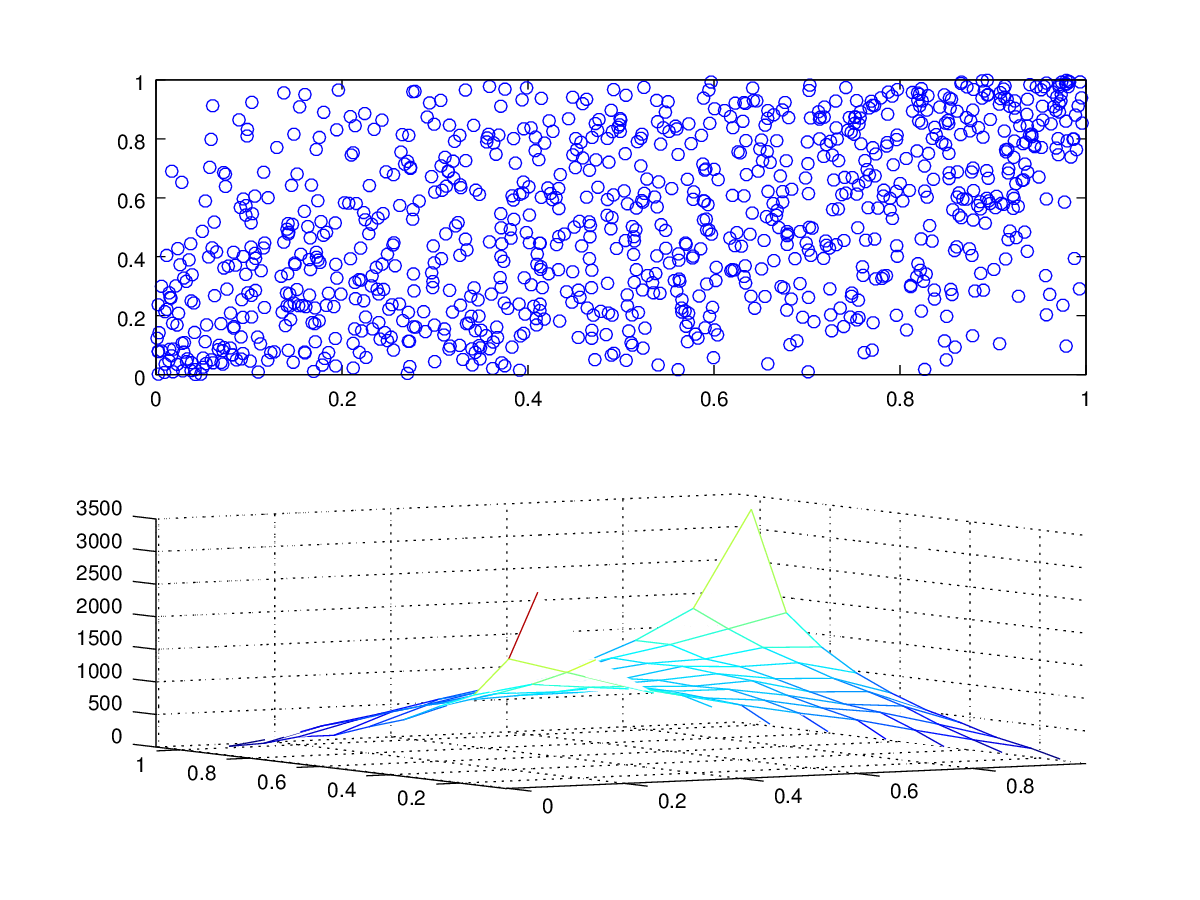
\includegraphics[scale = 0.50]{pictures/gaussian.eps}
\caption{Dvourozměrná Gausova kopula funkce s korelačním parametrem $\rho =   0.5$}
\end{figure}

\subsubsection{Odhad parametrů}

Gausova kopula je plně definována korelační maticí. Tu lze odhadnout pomocí Kendall pořadové korelace, kterou lze převést na klasickou korelaci $\rho$ pomocí vztahu
\begin{equation*}
\rho(X) = \sin\left(\frac{\pi}{2}\right)
\end{equation*}
Z jednotlivých párových korelací pak lze sestavit kompletní korelační matici. Takto zkonstruovaná matice nemusí být nutně pozitivně semidefinitní (i když tomu tak v praxi obvykle bývá), a proto je vhodné provést kontrolu a matici případně upravit.

Související funkce \textit{CalcKendallTau.m} je k dispozici v adresáři \textit{libs}.

Funkce \textit{FitGausianCopula.m} pro odhad parametrů Gausovy kopula funkce je k dispozici v adresáři \textit{Copulas}.

\subsubsection{Simulace}

Předpokládejme, že máme k dispozici korelační matici $\Sigma$, kterou jsme odhadli v předchozím kroku.

\begin{enumerate}
\item Pomocí Choleskyho dekompozice provedeme rozklad kovarianční matice na $\Sigma = \Sigma^{1/2} \Sigma^{1/2}$.
\item Vygenerujeme vektor $Z = (Z_1, Z_2, ..., Z_d)' \sim N(0, \Sigma)$ nezávislých standardních normálních veličin.
\item Vypočteme vektor $X = \Sigma^{1/2}Z$ korelovaných standardních normálních veličin, kde $X = (X_1, X_2, ..., X_d)$.
\item Vypočteme $U = \left(\Phi(X_1), \Phi(X_2), ..., \Phi(X_d)) \right)$, kde $\Phi$ je distribuční funkce standardního normálního rozdělení. Náhodný vektor $U$ sleduje Gausovu kopula funkci\footnote{Připomeňme, že Gausova kopula funkce je distribuční funkcí. Vektor $U$ tak lze chápat jako náhodný výběr z této distribuční funkce. To je ostatně smyslem výše popsané simulace.}.
\end{enumerate}

Související funkce \textit{SimulGausianCopula.m} je k dispozici v adresáři \textit{Copulas}.

\subsubsection{Asymptotická nezávislost ve chvostech}

Nechť $(X_1, X_2) := (\Phi^{-1}(U_1), \Phi^{-1}(U_2))$ tak, že $(X_1, X_2)$ sleduje dvourozměrné normální rozdělení se standardním normálním rozdělením jako marginální distribuční funkcí a korelací $\rho$. Koeficient závislosti v dolním chvostu této Gaussovy kopula funkce je
\begin{multline*}
\lambda = 2 \lim_{x \rightarrow 0^+} P(\Phi^{-1}(U_2) \le \Phi^{-1}(q) | \Phi^{-1}(U_1) = \Phi^{-1}(q))\\
= 2 \lim_{x \rightarrow -\infty} P(X_2 \le x | X_1 = x)
\end{multline*}
S využitím skutečnosti $X_2 | X_1 = x \sim N(\rho x, 1 - \rho^2)$\footnote{Nechť $X_1$ a $X_2$ jsou dvě nezávislé náhodné veličiny, které sledují standardizované normální rozdělení. Definujme $\epsilon_1 = X_1$ a $\epsilon_2 = \rho X_1 + \sqrt{1 + \rho^2}X_2$. Lze dokázat, že $\epsilon_1$ a $\epsilon_2$ jsou náhodné veličiny s korelací $\rho$, které sledují standardizované normální rozdělení. Platí
\begin{equation*}
E[\epsilon_2 | \epsilon_1 = \epsilon^*] = E[\rho \epsilon^* + x_2 \sqrt{1 - \rho^2}] = \rho \epsilon^*
\end{equation*}
\begin{equation*}
E[\epsilon_2^2 | \epsilon_1 = \epsilon^*] = E[(\rho \epsilon^*)^2 + 2 \rho \epsilon^* x_2(1 - \rho^2) + (1 - \rho^2)x_2^2] = (\rho \epsilon^*)^2 + (1 - \rho^2)
\end{equation*}
což implikuje
\begin{multline*}
D[\epsilon_2 | \epsilon_1 = \epsilon^*] = E[\epsilon_2^2 | \epsilon_1 = \epsilon^*] - E[\epsilon_2 | \epsilon_1 = \epsilon^*]^2\\
= (\rho \epsilon^*)^2 + (1 - \rho^2) - (\rho \epsilon^*)^2 = 1 - \rho^2
\end{multline*}
a proto $\epsilon_2 | \epsilon_1 = \epsilon^* \sim N(\rho \epsilon^*, 1 - \rho^2)$.} lze odvodit
\begin{equation*}
P(X_2 \le x | X_1 = x) = \Phi\left(\frac{x - \rho x}{\sqrt{1 - \rho^2}} \right) = \Phi \left(\frac{x \sqrt{1 - \rho}^2}{\sqrt{1 - \rho}\sqrt{1 + \rho}}\right) = \Phi \left(\frac{x \sqrt{1 - \rho}}{\sqrt{1 + \rho}} \right)
\end{equation*}
a proto
\begin{equation*}
\lambda = 2 \lim_{x \rightarrow -\infty} \Phi\left(\frac{x \sqrt{1 - \rho}}{\sqrt{1 + \rho}}\right) = 0
\end{equation*}
za předpokladu $\rho < 1$. Gausova kopula funkce je tedy asymptoticky nezávislá v obou chvostech a to bez ohledu na to, jak vysokou korelaci $\rho$ zvolíme.

\subsubsection{Omezení}

Ačkoliv je Gausova kopula funkce jednou z nejpoužívanějších, má řadu zásadních omezení.

Gausova kopula funkce patří do rodiny eliptických funkcí - jedná se tedy o symetrickou distribuční funkci. To znamená, že např. pravděpodobnost extrémního nárůstu cen akcií je shodná s pravděpodobností extrémně negativního poklesu. To je v rozporu s empirickým pozorováním, kdy pravděpodobnost extrémního poklesu je zpravidla výrazně vyšší než pravděpodobnost extrémního nárůstu.

Notoricky známým nedostatkem normálního rozdělení je nedostatečné podchycení případných tlustých chvostů. Z empirických dat je zřejmé, že právě tlusté chvosty jsou typická pro finanční data.

Jak jsme ukázali výše, dalším zásadním nedostatkem je skutečnost, že korelace mezi jednotlivými náhodnými veličinami se v chvostech Gausovy kopula funkce asymptoticky blíží nule. Pokud je tedy předmětem našeho zájmu vypočet value-at-risk, který se opírá o kvantily 99\% a vyšší, je Gausova kopula funkce nevhodná.

\subsection{Studentova kopula funkce}

Narozdíl od Gausovy kopula funkce umožňuje studentova kopula funkce částečně podchytit problematiku tlustých chvostů a to skrze parametr počet stupňů volnosti. Nicméně standardní studentova kopula funkce má pouze jeden takovýto parametr bez ohledu na dimenzi $d$. Podobně jako pro Gausovu kopula funkci jsou parametry studentovy kopula funkce relativně snadno odhadnutelné, což je jeden z hlavních důvodů její oblíbenosti v praxi.

\begin{figure}[htp]
\centering
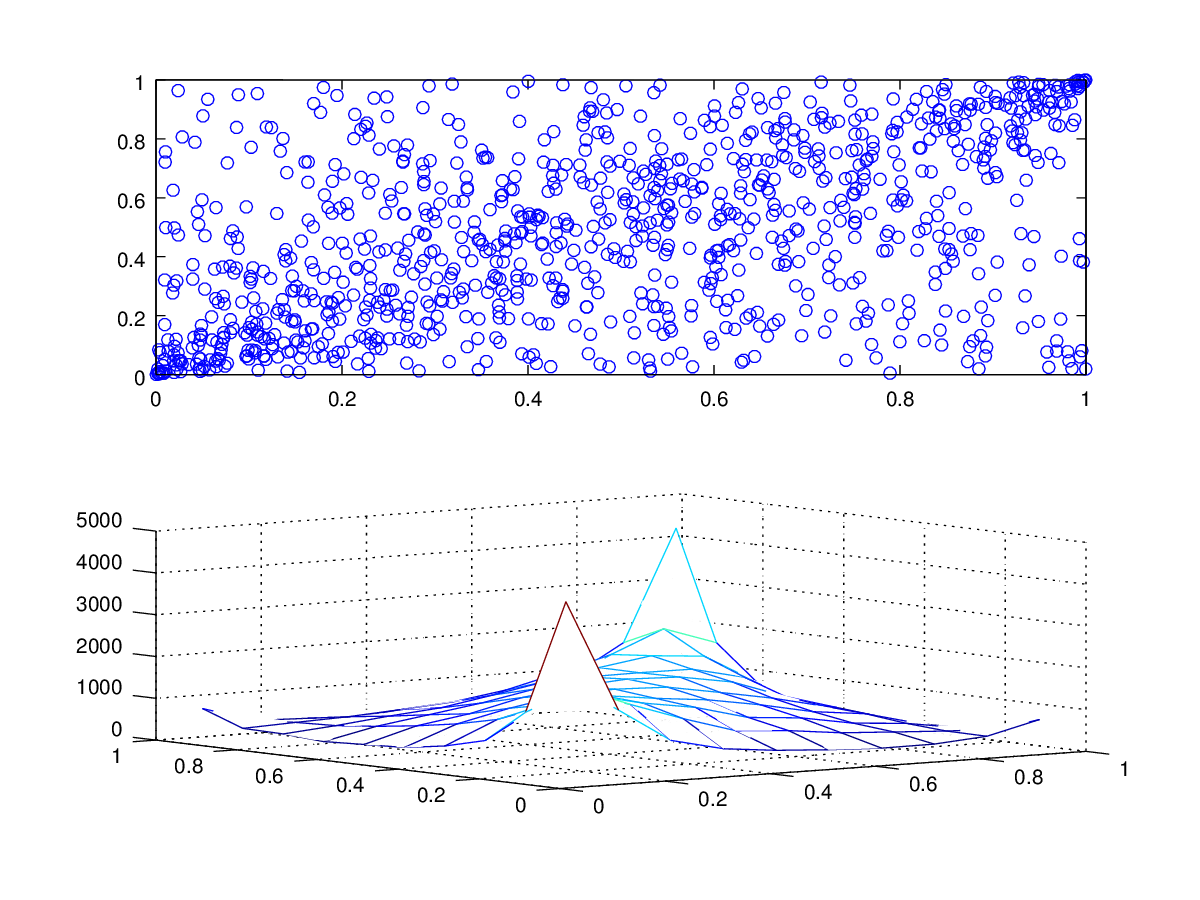
\includegraphics[scale = 0.50]{pictures/student.eps}
\caption{Dvourozměrná studentova kopula funkce s korelačním parametrem $\rho =   0.5$ a počtem stupňů volnosti $\nu = 2$}
\end{figure}

\subsubsection{Odhad parametrů}

V případě studentovy kopula funkce je třeba odhadnout kromě korelační matice také počet stupňů volnosti. Stejně jako v případě Gausovy kopula funkce lze korelační matice odhadnout pomocí Kendall pořadové korelace. Počet stupňů volnosti lze odhadnout pomocí MLE maxilizací funkce
\begin{equation*}
\max_{\nu} \sum_{i = 1}^N \ln \Big(c_{\nu, \Sigma}^t(u_i)\Big)
\end{equation*}
kde $u_i$ představuje vektor dimenze $d$ obsahující kvantily $i$-tého pozorování, $N$ představuje celkový počet pozorování a $c_{\nu, \Sigma}^t(u_i)$ je hustotu pravděpodobnosti studentovy kopula funkce definovanou jako
\begin{equation*}
c_{\nu, \Sigma}^t(u_i) = \frac{f_{\nu, \Sigma}(t_{v}^{-1}(u_{i1}), t_{v}^{-1}(u_{i2}), ..., t_{v}^{-1}(u_{id}))}{\prod_{j = 1}^d f_{\nu}(t_{\nu})^{-1}(u_{ij})}, ~~~ u \in (0, 1)^d
\end{equation*}
kde $f_{\nu, \Sigma}$ je sdružená hustota pravděpodobnosti $d$-rozměrného studentova rozdělení s $\nu$ stupni volnosti a korelační maticí $\Sigma$ a $f_{\nu}$ je hustota pravděpodobnosti jednorozměrného studentova rozdělení s $\nu$ stupni volnosti. 

Funkce \textit{FitStudentCopula2.m} pro odhad parametrů studentovy kopula funkce je k dispozici v adresáři \textit{Copulas}.

\subsubsection{Simulace}

Předpokládejme, že máme k dispozici korelační matici $\Sigma$ a počet stupňů volnosti, které jsme odhadli v předchozím kroku.

\begin{enumerate}
\item Pomocí Choleskyho dekompozice provedeme rozklad kovarianční matice na $\Sigma = \Sigma^{1/2} \Sigma^{1/2}$.
\item Vygenerujeme vektor $Z = (Z_1, Z_2, ..., Z_d)' \sim N(0, \Sigma)$ nezávislých standardních normálních veličin.
\item Vypočteme vektor $X = \Sigma^{1/2}Z$ korelovaných standardních normálních veličin, kde $X = (X_1, X_2, ..., X_d)$.
\item Vygenerujeme náhodnou veličinu $Y$ z $\chi^2$ pravděpodobnostního rozdělení s parametrem $\nu$.
\item Vypočteme vektor $T = \left( \frac{X_1}{\nu / \sqrt{Y}}, \frac{X_2}{\nu / \sqrt{Y}}, \frac{X_d}{\nu / \sqrt{Y}} \right)$.
\item Vypočteme $U = \left(t_{\nu}^{cdf}(T_1), t_{\nu}^{cdf}(t_2), ...,  t_{\nu}^{cdf}(Z_d)) \right)$, kde $t_{\nu}^{cdf}$ je distribuční funkce studentova rozdělení s $\nu$ stupni volnosti. Náhodný vektor $U$ sleduje studentovu kopula funkci s korelační maticí $\Sigma$ a $\nu$ stupni volnosti.
\end{enumerate}

Související funkce \textit{SimulStudentCopula.m} je k dispozici v adresáři \textit{Copulas}.

\subsubsection{Asymptotická závislost v chvostech}

Uvažujme $(X_1, X_2) := (t_{\nu}^{-1}(U_1), t_{\nu}^{-1}(U_2))$, kde $t_{\nu}$ označuje distribuční funkci jednorozměrného studendova rozdělení s $\nu$ stupni volnosti. Proto $(X_1, X_2) \sim t_2(\nu, 0, P)$, kde $P$ je korelační matice s prvkem $\rho$ mimo hlavní diagonálu. Lze dovodit, že podmíněná pravděpodobnost pro $X_1 = x$ zdvourozměrného studentova rozdělení je
\begin{equation*}
\left(\frac{v + 1}{v + x^2}\right)^{\frac{1}{2}} \frac{X_2 - \rho x}{\sqrt{1 - \rho^2}} \sim t_{v + 1}
\end{equation*}
Podobnou argumentací jako v případě Gausovy kopula funkce lze dokázat
\begin{equation*}
\lambda = 2 t_{v + 1} \left(-\sqrt{\frac{(v + 1)(1 - \rho)}{1 + \rho}}\right)
\end{equation*}
Za předpokladu $\rho > - 1$ tedy studentova kopula funkce vykazuje závislost ve svém horním i dolním chvostu.

\subsubsection{Omezení}

Na studentovu kopula funkci lze pohlížet jako na zobecnění Gausovy kopula funkce. Přesto (anebo spíše právě proto) sdílí s Gausovou kopula funkcí řadu omezení.

Stejně jako Gausova kopula funkce patří studentova kopula funkce do rodiny eliptických funkcí a jedná se tedy o symetrickou distribuční funkci. Empirická data však hypotézu o symetrii příliš nepodporují. Tomuto problému se lze vyhnout pomocí tzv. sešikmené studentovy kopula funkce, která je rozšířením původního modelu. Odhad parametrů sešikmení je však časově poměrně náročný.

Tlusté chvosty jsou částečně podchyceny skrze počet stupňů volnosti. Nicméně základní studentova kopula funkce má pouze jeden takovýto parametr bez ohledu na svou dimenzi. Problém lze částečně obejít rozšířením modelu, kdy pro každou dimenzi definujeme vlastní počet stupňů volnosti - hovoříme o tzv. studentově kopula funkcí s vícero stupni volnosti. Kalibrace této kopula funkce je však časově náročná, a proto se v praxi příliš nepoužívá. Funkce \textit{FitStudentMDoF.m} a \textit{SimulStudentMDoF.m}, které slouží ke kalibraci resp. k simulaci tohoto typu kopula funkce jsou k dispozici v adresáři \textit{Copulas}.

Na rozdíl od Gausovy kopula funkce se korelace v chvostech asymptoticky neblíží nule. To však neznamená, že modelová korelace odpovídá skutečné korelaci. Teoretickým řešením je sloučení dvou výše uvedených rozšíření v tzv. sešikmenou studentovu kopula funkci s vícero stupni volnosti, kdy skrze větší počet parametrů získáme potřebnou flexibilitu. V praxi však tento přístup naráží na problém s kalibrací, která je nestabilní a navíc velmi časově náročná.

\subsection{Archimediánské kopula funkce}

Obecná Archimediánská kopula funkce je definována jako
\begin{equation}
C(u_1, u_2) = \phi^{-1}\left(\phi(u_1) + \phi(u_2)\right)
\end{equation}
kde $\phi$ je klesající funkce, která mapuje z $[0, 1]$ do $[0, \infty]$ a splňuje $\phi(0) = \infty$ a $\phi(1) = 0$. Funkci $\phi$ nazýváme kopula generátorem. Z (2.1) vyplývá, že Archimediánské kopule jsou dvourozměrné. Existují také vícerozměrné varianty Archimediánských kopula funkcí, ty však nejsou předmětem tohoto textu. Do rodiny Archimediánských kopula funkcí patří Claytonova, Gumbelova a Frankova kopula funkce.

\subsubsection{Claytonova kopula funkce}

Dvourozměrná Claytonova kopula funkce má tvar
\begin{equation*}
C_{\theta}(u_1, u_2) = (u_1^{-\theta} + u_2^{-\theta} - 1)^{-\frac{1}{\theta}}, ~~~ 0 < \theta < \infty
\end{equation*}
Pro $\theta \rightarrow 0$ získáme nezávislou kopula funkci; pro $\theta \rightarrow \infty$ získáme komonotonickou kopula funkci. Parametr $\theta$ tak měří sílu závislosti v rámci kopula funkce.

\begin{figure}[htp]
\centering
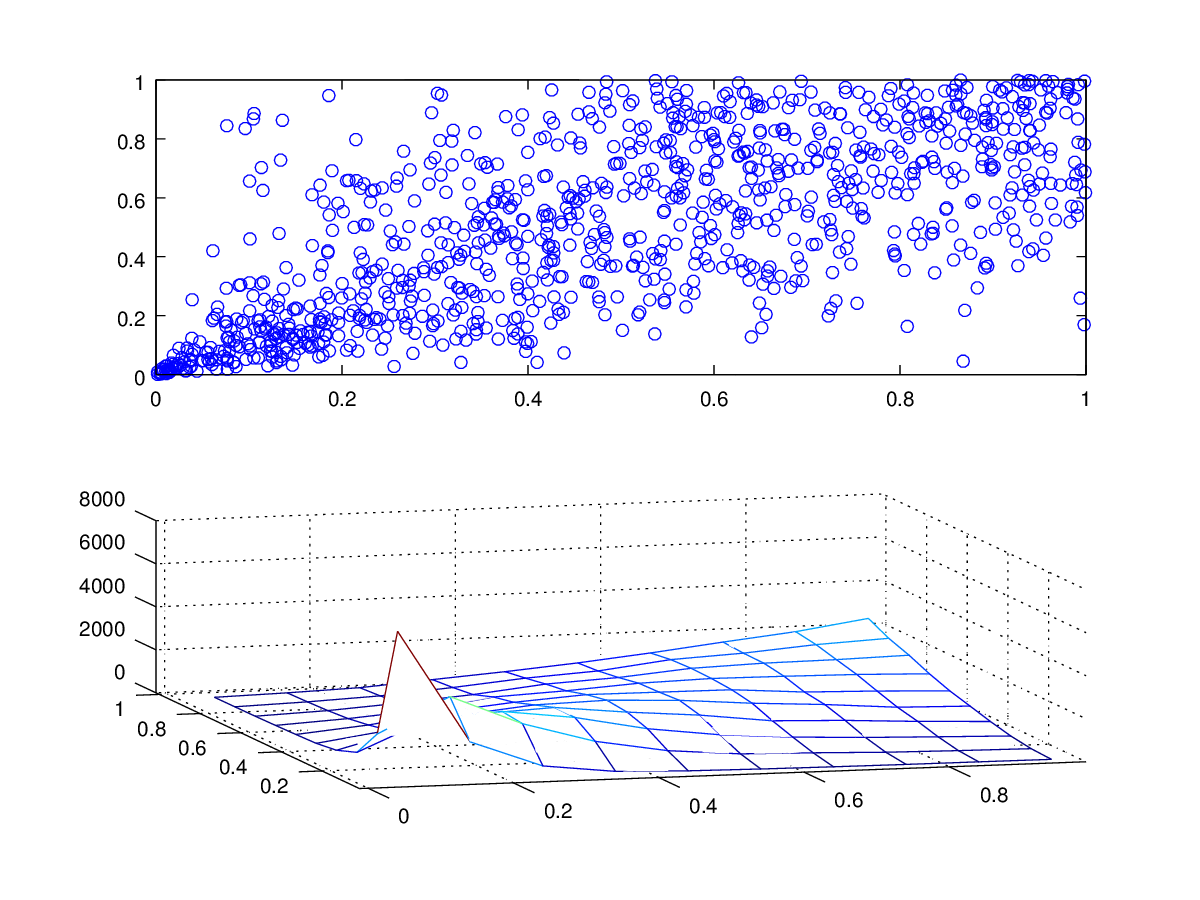
\includegraphics[scale = 0.50]{pictures/clayton.eps}
\caption{Dvourozměrná Claytonova kopula funkce s parametrem $\theta = 2$}
\end{figure}

Pro kalibraci Claytonovy kopula funkce stačí odhadnout parametr $\theta$. Mezi $\theta$ a Kendall pořadovou korelací $\rho_{\tau}$ existuje vztah
\begin{equation}
\rho_{\tau} = \frac{\theta}{\theta + 2}
\end{equation}
Prvním krokem kalibrace je tedy výpočet Kendall pořadové korelace (viz. výše), na který navazuje výpočet parametru $\theta$ pomocí inverze (2.2). Příslušná funkce \textit{FitClaytonCopula.m} je k dispozici v adresáři \textit{Copulas}.

Simulace z Claytonovy kopule probíhá v následujících krocích.
\begin{enumerate}
\item Vygenerujeme náhodnou veličinu $V \sim Ga(1/\theta, 1)$, kde $\theta > 0$ a $Ga(\alpha, \beta)$ je pravděpodobnostní rozdělení gamma s hustotou pravděpodobnosti
\begin{equation*}
f(x) = \frac{\beta^{\alpha}}{\Gamma(\alpha)}x^{\alpha - 1}e^{-\beta x}, ~~~ x > 0, \alpha > 0, \beta > 0
\end{equation*}
kde $\Gamma(\alpha) = \int_0^{\infty} x^{\alpha - 1}e^{-x}dx, ~~~ \alpha > 0$. Distribuční funkce náhodné veličiny $V$ má Laplace transformaci $\hat{G}(t) = (1 + t) ^ {-\frac{1}{\theta}}$.
\item Vygenerujeme nezávislé uniformní náhodné veličiny $X = (X_1, X_2)$.
\item Vypočteme $U = \left(\hat{G}(-\ln(X_1)/V), \hat{G}(-\ln(X_2)/V)\right)$. Dvourozměrný náhodný vektor $U$ je výběrem z Claytonovy kopula funkce.
\end{enumerate}
Funkci \textit{SimulClaytonCopula.m} pro simulaci z Clayton kopula funkce naleznete v adresáři \textit{Copulas}.

\subsubsection{Gumbelova kopula funkce}

Dvourozměrná Gumbelova kopula funkce má tvar
\begin{equation*}
C_{\theta}(u_1, u_2) = e^{-\left((-\ln(u_1))^{\theta} + (-\ln(u_2))^{\theta}\right)^{\frac{1}{\theta}}}, ~~~ 1 \le \theta < \infty
\end{equation*}
Jestliže $\theta = 1$, získáme nezávislou kopula funkci; jestliže $\theta \rightarrow \infty$, získáme komonotonickou kopula funkci. Parametr $\theta$ tak stejně jako v případě Claytonovy kopula funkce vyjadřuje míru závislosti.

\begin{figure}[htp]
\centering
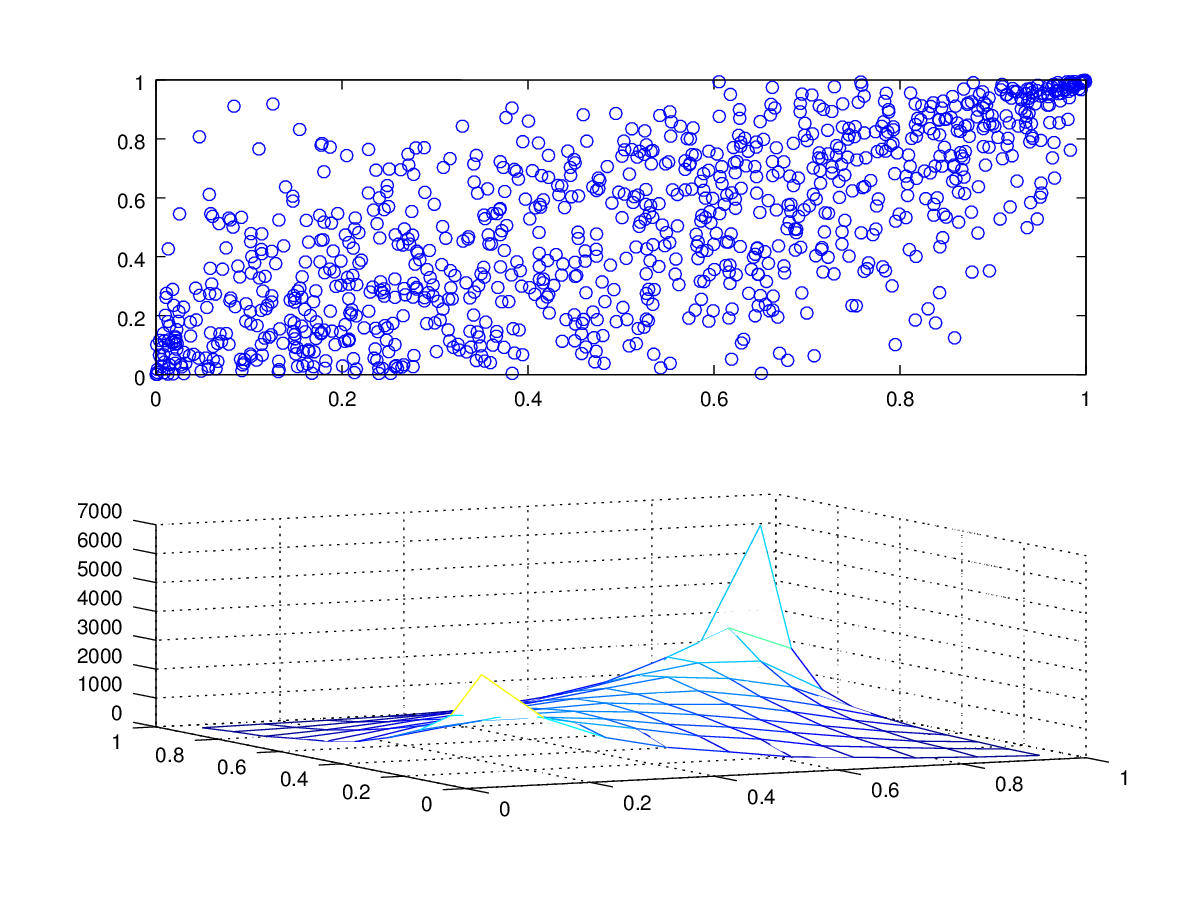
\includegraphics[scale = 0.50]{pictures/gumbel.eps}
\caption{Dvourozměrná Gumbelova kopula funkce s parametrem $\theta = 2$}
\end{figure}

Gumbelova kopula funkce je plně definována parametrem $\theta$. Stejně jako v případě Claytonovy kopula funkce existuje vztah mezi parametrem $\theta$ a Kendall pořadovou korelací $\rho_{\tau}$.
\begin{equation*}
\rho_{\tau} = \frac{\theta}{\theta + 2}
\end{equation*}
Pro kalibraci tedy nejprve stačí vypočíst Kendall pořadovou korelaci a z ní následně odvodit parametr $\theta$. Potřebná funkce \textit{FitGumbelCopula.m} je k dispozici v adresáři \textit{Copulas}.

Simulace sleduje podobné kroky jako v případě Claytonovy kopula funkce.
\begin{enumerate}
\item Vygenerujeme stabilní náhodnou veličinu $V \sim St(1 / \theta, 1, \gamma, 0)$, kde $\gamma = (cos(\pi/2\theta))^{\theta}$ a $\theta > 0$. Distribuční funkce náhodné veličiny $V$ má Laplace transformaci $\hat{G}(t) = e^{-t^{1/\theta}}$.
\item Vygenerujeme nezávislé uniformní náhodné veličiny $X = (X_1, X_2)$.
\item Vypočteme $U = \left(\hat{G}(-\ln(X_1)/V), \hat{G}(-\ln(X_2)/V)\right)$. Dvourozměrný náhodný vektor $U$ je výběrem z Gumbelovy kopula funkce.
\end{enumerate}

\subsubsection{Frankova kopula funkce}

Dvourozměrná Frankova kopula funkce má tvar
\begin{equation*}
C_{\theta}(u_1, u_2) = -\frac{1}{\theta}\ln \left(1 + \frac{(e^{-\theta u_1} - 1)(e^{-\theta u_2})}{e^{-\theta} - 1} \right) ~~~ \theta \in R - \{0\}
\end{equation*}

\begin{figure}[htp]
\centering
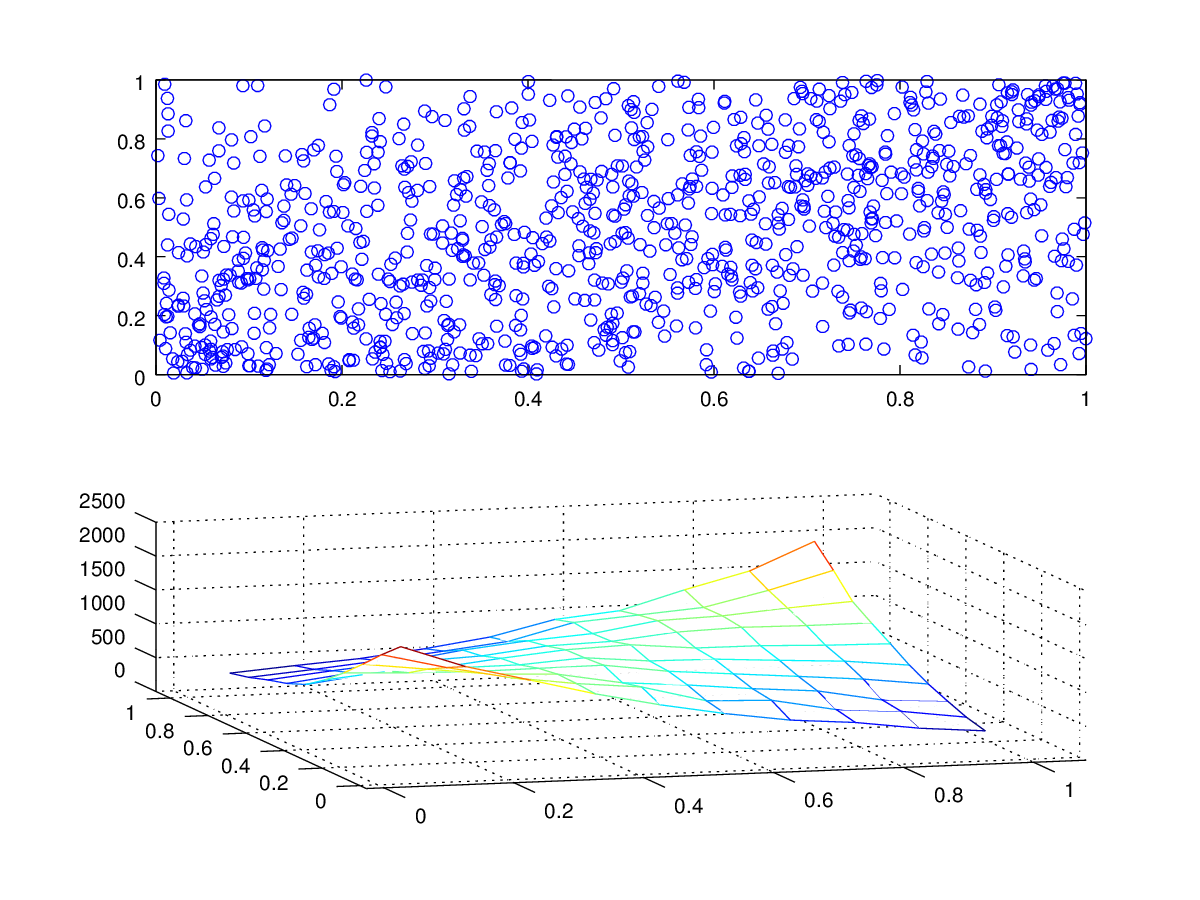
\includegraphics[scale = 0.50]{pictures/frank.eps}
\caption{Dvourozměrná Frankova kopula funkce s parametrem $\theta = 2$}
\end{figure}

Prvním krokem kalibrace Frankovy kopula funkce je výpočet Kendall pořadové korelace, ze které pomocí vztahu
\begin{equation*}
\rho_{\tau} = 1 - 4 \theta ^ {-1}\left(1 - D_1(\theta)\right)
\end{equation*}
kde $D_1(\theta) = \theta ^ {-1} \int_0^{\theta}\frac{t}{e^t - 1}dt$ je Debye funkce. Parametr $\theta$ nelze z tohoto vztahu vyjádřit přímo, a proto je třeba vypočíst iterativně např. pomocí Newtonovy metody.

Simulace z Frankovy kopula funkce probíhá v následujících krocích.
\begin{enumerate}
\item Vygenerujeme diskrétní náhodnou veličinu $V$ s pravděpodobnostní funkcí $p(k) = P(V = k) = \frac{(1 - e^{-\theta})^k}{k \theta}$ pro $k = 1, 2, ...$  a $\theta > 0$. Laplace transformace odpovídající distribuční funkce má tvar $\hat{G}(t) = \frac{1}{\theta} \ln \left(e^{-t}(1 - e^{-\theta}) - 1\right)$.
\item Vygenerujeme nezávislé uniformní náhodné veličiny $X = (X_1, X_2)$.
\item Vypočteme $U = \left(\hat{G}(-\ln(X_1)/V), \hat{G}(-\ln(X_2)/V)\right)$. Dvourozměrný náhodný vektor $U$ je výběrem z Frankovy kopula funkce.
\end{enumerate}

\chapter{Použitá literatura}

\begin{enumerate}
\item Coping with Copulas - Thorsten Schmidt; Department of Mathematics, University of Leipzig December 2006
\item The Estimation of Copulas: Theory and Practice; Arthur Charpentier, Jean-David Fermanian, Olivier Scaillet; September 2006
\item Quantitative Risk Management - Alexander J. McNeil, Rudiger Frey, Paul Embrechts; Princenton University Press 2005
\item The Bivariate Normal Copula - Christian Meyer, December 15, 2009
\item The t Copula and Related Copulas - Stefano Demarta, Alexander J. McNeil; Department of Mathematics, Federal Institute of Technology ETH Zentrum; May 2004
\item The t Copula with Multiple Parameters of Degree of Freedom: Bivariate Characteristics and Applications to Risk Management; Xiaolin Luo, Pavel V. Shevchenko; 28 May 2009
\item The Asymetric t-Copula with Individual Degress of Freedom; Christ Church; University of Oxford, 2012
\item Copula Modelling: An Introduction for Practitioners; Pravin K. Trivedi, David M. Zimmer; Foundantions and Trends in Econometrics 2005
\item ML Estimation of the t Distribution Using EM and its Extensions, ECM and ECME; Chuanhai Liu, Donald B. Rubin; Harvard University
\item Stable Distributions, Models for Heavy Tailed Data; John P. Nolan; Math/Stat Department of American University; July 28, 2014
\item SAS/ETS(R) 9.3 User's Guide - The Copula Procedure - Archimedian Copulas
\item Kendall tau rank correlation coefficient; Wikipedia
\item Kernel (statistics); Wikipedia
\item Kernel density estimation; Wikipedia
\item Kernel smoother; Wikipedia
\end{enumerate}


\end{document}
